% Options for packages loaded elsewhere
\PassOptionsToPackage{unicode}{hyperref}
\PassOptionsToPackage{hyphens}{url}
%
\documentclass[
  Letterpaper,
]{scrbook}

\usepackage{amsmath,amssymb}
\usepackage{iftex}
\ifPDFTeX
  \usepackage[T1]{fontenc}
  \usepackage[utf8]{inputenc}
  \usepackage{textcomp} % provide euro and other symbols
\else % if luatex or xetex
  \usepackage{unicode-math}
  \defaultfontfeatures{Scale=MatchLowercase}
  \defaultfontfeatures[\rmfamily]{Ligatures=TeX,Scale=1}
\fi
\usepackage{lmodern}
\ifPDFTeX\else  
    % xetex/luatex font selection
    \setmainfont[]{Georgia}
\fi
% Use upquote if available, for straight quotes in verbatim environments
\IfFileExists{upquote.sty}{\usepackage{upquote}}{}
\IfFileExists{microtype.sty}{% use microtype if available
  \usepackage[]{microtype}
  \UseMicrotypeSet[protrusion]{basicmath} % disable protrusion for tt fonts
}{}
\makeatletter
\@ifundefined{KOMAClassName}{% if non-KOMA class
  \IfFileExists{parskip.sty}{%
    \usepackage{parskip}
  }{% else
    \setlength{\parindent}{0pt}
    \setlength{\parskip}{6pt plus 2pt minus 1pt}}
}{% if KOMA class
  \KOMAoptions{parskip=half}}
\makeatother
\usepackage{xcolor}
\usepackage[paperwidth=6in,paperheight=9in]{geometry}
\setlength{\emergencystretch}{3em} % prevent overfull lines
\setcounter{secnumdepth}{5}
% Make \paragraph and \subparagraph free-standing
\makeatletter
\ifx\paragraph\undefined\else
  \let\oldparagraph\paragraph
  \renewcommand{\paragraph}{
    \@ifstar
      \xxxParagraphStar
      \xxxParagraphNoStar
  }
  \newcommand{\xxxParagraphStar}[1]{\oldparagraph*{#1}\mbox{}}
  \newcommand{\xxxParagraphNoStar}[1]{\oldparagraph{#1}\mbox{}}
\fi
\ifx\subparagraph\undefined\else
  \let\oldsubparagraph\subparagraph
  \renewcommand{\subparagraph}{
    \@ifstar
      \xxxSubParagraphStar
      \xxxSubParagraphNoStar
  }
  \newcommand{\xxxSubParagraphStar}[1]{\oldsubparagraph*{#1}\mbox{}}
  \newcommand{\xxxSubParagraphNoStar}[1]{\oldsubparagraph{#1}\mbox{}}
\fi
\makeatother


\providecommand{\tightlist}{%
  \setlength{\itemsep}{0pt}\setlength{\parskip}{0pt}}\usepackage{longtable,booktabs,array}
\usepackage{calc} % for calculating minipage widths
% Correct order of tables after \paragraph or \subparagraph
\usepackage{etoolbox}
\makeatletter
\patchcmd\longtable{\par}{\if@noskipsec\mbox{}\fi\par}{}{}
\makeatother
% Allow footnotes in longtable head/foot
\IfFileExists{footnotehyper.sty}{\usepackage{footnotehyper}}{\usepackage{footnote}}
\makesavenoteenv{longtable}
\usepackage{graphicx}
\makeatletter
\newsavebox\pandoc@box
\newcommand*\pandocbounded[1]{% scales image to fit in text height/width
  \sbox\pandoc@box{#1}%
  \Gscale@div\@tempa{\textheight}{\dimexpr\ht\pandoc@box+\dp\pandoc@box\relax}%
  \Gscale@div\@tempb{\linewidth}{\wd\pandoc@box}%
  \ifdim\@tempb\p@<\@tempa\p@\let\@tempa\@tempb\fi% select the smaller of both
  \ifdim\@tempa\p@<\p@\scalebox{\@tempa}{\usebox\pandoc@box}%
  \else\usebox{\pandoc@box}%
  \fi%
}
% Set default figure placement to htbp
\def\fps@figure{htbp}
\makeatother
% definitions for citeproc citations
\NewDocumentCommand\citeproctext{}{}
\NewDocumentCommand\citeproc{mm}{%
  \begingroup\def\citeproctext{#2}\cite{#1}\endgroup}
\makeatletter
 % allow citations to break across lines
 \let\@cite@ofmt\@firstofone
 % avoid brackets around text for \cite:
 \def\@biblabel#1{}
 \def\@cite#1#2{{#1\if@tempswa , #2\fi}}
\makeatother
\newlength{\cslhangindent}
\setlength{\cslhangindent}{1.5em}
\newlength{\csllabelwidth}
\setlength{\csllabelwidth}{3em}
\newenvironment{CSLReferences}[2] % #1 hanging-indent, #2 entry-spacing
 {\begin{list}{}{%
  \setlength{\itemindent}{0pt}
  \setlength{\leftmargin}{0pt}
  \setlength{\parsep}{0pt}
  % turn on hanging indent if param 1 is 1
  \ifodd #1
   \setlength{\leftmargin}{\cslhangindent}
   \setlength{\itemindent}{-1\cslhangindent}
  \fi
  % set entry spacing
  \setlength{\itemsep}{#2\baselineskip}}}
 {\end{list}}
\usepackage{calc}
\newcommand{\CSLBlock}[1]{\hfill\break\parbox[t]{\linewidth}{\strut\ignorespaces#1\strut}}
\newcommand{\CSLLeftMargin}[1]{\parbox[t]{\csllabelwidth}{\strut#1\strut}}
\newcommand{\CSLRightInline}[1]{\parbox[t]{\linewidth - \csllabelwidth}{\strut#1\strut}}
\newcommand{\CSLIndent}[1]{\hspace{\cslhangindent}#1}

\makeatletter
\@ifpackageloaded{bookmark}{}{\usepackage{bookmark}}
\makeatother
\makeatletter
\@ifpackageloaded{caption}{}{\usepackage{caption}}
\AtBeginDocument{%
\ifdefined\contentsname
  \renewcommand*\contentsname{Table of contents}
\else
  \newcommand\contentsname{Table of contents}
\fi
\ifdefined\listfigurename
  \renewcommand*\listfigurename{List of Figures}
\else
  \newcommand\listfigurename{List of Figures}
\fi
\ifdefined\listtablename
  \renewcommand*\listtablename{List of Tables}
\else
  \newcommand\listtablename{List of Tables}
\fi
\ifdefined\figurename
  \renewcommand*\figurename{Figure}
\else
  \newcommand\figurename{Figure}
\fi
\ifdefined\tablename
  \renewcommand*\tablename{Table}
\else
  \newcommand\tablename{Table}
\fi
}
\@ifpackageloaded{float}{}{\usepackage{float}}
\floatstyle{ruled}
\@ifundefined{c@chapter}{\newfloat{codelisting}{h}{lop}}{\newfloat{codelisting}{h}{lop}[chapter]}
\floatname{codelisting}{Listing}
\newcommand*\listoflistings{\listof{codelisting}{List of Listings}}
\makeatother
\makeatletter
\makeatother
\makeatletter
\@ifpackageloaded{caption}{}{\usepackage{caption}}
\@ifpackageloaded{subcaption}{}{\usepackage{subcaption}}
\makeatother

\usepackage{bookmark}

\IfFileExists{xurl.sty}{\usepackage{xurl}}{} % add URL line breaks if available
\urlstyle{same} % disable monospaced font for URLs
\hypersetup{
  pdftitle={The Human Element},
  pdfauthor={Sami Karam and Richard Sprague},
  hidelinks,
  pdfcreator={LaTeX via pandoc}}


\title{The Human Element}
\usepackage{etoolbox}
\makeatletter
\providecommand{\subtitle}[1]{% add subtitle to \maketitle
  \apptocmd{\@title}{\par {\large #1 \par}}{}{}
}
\makeatother
\subtitle{Why AI Will Enhance, Not Replace}
\author{Sami Karam and Richard Sprague}
\date{2025-01-24}

\begin{document}
\frontmatter
\maketitle

\renewcommand*\contentsname{Table of contents}
{
\setcounter{tocdepth}{2}
\tableofcontents
}

\mainmatter
\bookmarksetup{startatroot}

\chapter*{Preface}\label{preface}
\addcontentsline{toc}{chapter}{Preface}

\markboth{Preface}{Preface}

This is an initial placeholder for a 75,000 word book.

Current word count = 20498

This is the preface

test 12345678

\bookmarksetup{startatroot}

\chapter*{Introduction}\label{introduction}
\addcontentsline{toc}{chapter}{Introduction}

\markboth{Introduction}{Introduction}

In 2021, a team of music historians, musicologists, composers and
computer scientists gathered in\ldots{} to undertake a task that had
never been attempted before: to complete Beethoven's tenth symphony with
the help of Artificial Intelligence. Beethoven had started composing the
symphony but had died in 1827 before making much progress. He only left
behind a few musical sketches, not a substantive draft on which the team
could easily build. Nonetheless, the team trained a computer on
Beethoven's entire body of work and then let AI do the rest of the work,
the composing of the entire symphony.

This is the typical way that AI works, in two main steps: firt ``to
learn'' and then ``to do''. An AI program has to first learn or
``train'' from an existing database everything that it can learn that is
relevant to the planned project. This is the training phase. Then the AI
program has to do or respond to a request to use what it has learned
during the training phase to deliver a response or an output. This is
the inference phase.

This is exactly what the \ldots{} team did. They trained AI on
Beethoven's symphonies and other musical pieces, as well as the early
sketches he had started for the tenth symphony, and then asked the AI
program to create the rest of the symphony based on what it had learned
during the training phase.

We start with this project because it neatly summarizes common
aspirations about AI. Many people do expect AI to eventually replace the
vast majority of human work. And here was an example with a team of
professionals training a machine to replace, or at least replicate, the
work of a human, albeit a genius and not an ordinary human.

There were much pomp and expectation around the project and the team
announced that the tenth symphony created by AI would be released in a
world premiere performance in Bonn, Germany, on October 9, 2021. When
the day came, \ldots{}

In the subsequent days and months, a consensus gradually formed about
the AI generated tenth symphony. And it was this: the music did sound
like Beethoven in many parts, but it lacked the ultimate ingredients
that made other symphonies masterpieces: passion, spirit, a tangible
human touch. Instead the AI tenth sounded mechanical and betrayed its
genesis by being too repetitive in the wrong places. In short, it was
precise and competent in the way of a robot, but it was ultimate
deficient for its inability to convey passion, to elevate and to inspire
listeners.

In our readings about the AI generated symphony, we looked at a large
number of opinions by experts from all walks of life. But one in
particular from Jan\ldots{} summarizes, in our view, the central reason
that the AI-generated tenth symphony fell short of actual
Beethoven-created symphonies. It was not only that it was mechanical and
repetitive. Perhaps these flaws could have been fixed in a subsequent
iteration. Nor was it that\ldots{} In the end, as J\ldots{} put it, the
tenth symphony fails to stir us for one main reason which is that
listeners ``want to see the human do it.''

Humans want to see other humans do it. These eight words sum up the
thesis of this book. And from them, we derive our belief that AI can be
a very effective assistant to humans in a large number of tasks but it
will never satisfactorily replace humans. Leadership and teamwork
require the input and inspiration imparted by a leader and by team
mates, and a robot, or AI-trained program, will never be able to provide
that human input and this inspiration.

This is the right time to have this conversation because the AI
revolution has spawned two competing narratives, both fundamentally
wrong. The doomsayers warn of widespread job displacement as artificial
intelligence becomes increasingly capable of performing human tasks. The
techno-utopians promise a future where AI solves humanity's greatest
challenges, freeing us from mundane work. But the reality emerging from
actual AI implementations tells a different story -- one where
artificial intelligence enhances rather than replaces human
capabilities. This means that the doomsayers are wrong because the
optimal completion of a task will remain elusive without the work of
humans using AI. And it also means that the techno-utopians are also
wrong because AI will not harness the creativity that is need to solve
on its own our greatest challenges.

Our own view is that AI is best seen as a force multiplier, and a
formidable one. Humanity has developed many force multipliers through
its history and they have all added to the productivity of humans and to
the wealth of society. And now humanity will develop yet another, and
perhaps the most powerful of all, force multiplier that will similarly
boost productivity and raise living standards.

This is not to say that all jobs will be preserved. Of course, there
will be much disruption and dislocation. Many jobs will completely
disappear or will be completely taken over by AI, but AI will be in most
cases a very competent and very efficient assistant, not a leader or
conductor of the proceedings. It is true at the same time that large
numbers of people will need to retrain to do other jobs, but this has
often be true in our modern society. It may well be that the numbers
will be larger this time around, but they were also larger last time
than they had been the previous time. Human progress is inherently
destructive of jobs that can be replaced by machine. There are millions
of robots today that perform the tasks that used to be done by human
factory workers only a few decades ago. This has always been the march
of technology. AI may be faster than previous revolutions, but then its
rewards will also be faster and richer.

Talking more practically, we have already observed a pattern across
industries that supports our thesis: the most successful AI applications
are those that augment human judgment rather than attempt to replicate
it. Here we draw on our long experiences in finance and technology. We
see that from financial trading desks to hospital diagnostic centers,
from military command posts to creative studios, the winning formula
consistently involves keeping humans ``in the loop'' while leveraging
AI's computational capabilities. We are in the early days of AI but our
view is that this will remain true with future AI systems that are far
more developed than today's.

Previous technological revolutions followed similar paths. There was
much concern among bank tellers when ATMs were first introduced that the
job of a human teller was going to disappear. This was a rational fear.
Why wait in line to see a teller if you can just make deposits and
withdrawals at an ATM? And from the bank's point of view, why employ
tellers when you can deploy ATMs at a much lower cost? It turned however
that people still needed human tellers for transactions that went beyond
simple deposits and withdrawals. But another dynamic proved even more
revealing. Because banks were able to reduce the number of tellers per
branch and were also able to reduce their costs thanks to other
technological advances, they were ultimately able to open more branches,
each of which required a minimal number of human tellers. The net result
is that the total number of people employed as tellers was in fact
larger after ATMs were introduced than before they were introduced.

The same experience was repeated in other fields. Computer-aided design
tools were expected to replace architects; instead, they enhanced
architects' ability to explore creative possibilities through new
technology and it allowed architecture firms to hire more architects.

One key difference today may be the pace and scope of change that AI
enables.

What makes AI unique is its ability to process vast amounts of data and
recognize patterns that humans might miss. But this capability,
impressive as it is, remains fundamentally different from human
intelligence. AI can analyze millions of medical images to flag
potential anomalies, but it takes a doctor's judgment to interpret these
findings in the context of a patient's overall health. AI can process
thousands of financial data points per second, but it takes a human
analyst to understand how changing geopolitical dynamics might affect
market sentiment.

This book challenges both the fear-mongering and the hype around AI.
Instead, we present a framework for understanding how AI can enhance
human capabilities across industries. Drawing on real-world case studies
and our own experience implementing AI solutions, we demonstrate why
keeping humans central to decision-making leads to better outcomes than
pursuing full automation. For business leaders, this book offers
practical guidance on implementing AI in ways that augment rather than
replace human workers. For investors, we provide frameworks for
evaluating AI companies based on their approach to human-AI
collaboration. For policymakers, we outline principles for governing AI
development while preserving human agency and judgment.

The coming decades will see artificial intelligence transform every
industry. But this transformation will not follow the simple pattern of
automation and replacement that many predict. Instead, we are entering
an era of enhancement, where human capabilities are amplified by AI
rather than superseded by it. Understanding this distinction -- and its
implications for business strategy, investment decisions, and policy
choices -- will be crucial for navigating the AI revolution.

The future belongs not to those who try to replicate human intelligence,
but to those who find ways to enhance it. This is the human element in
the AI revolution.

\bookmarksetup{startatroot}

\chapter{The False Binary: Why AI Won't Replace Human
Work}\label{the-false-binary-why-ai-wont-replace-human-work}

How both AI doomsayers and utopians miss the fundamental nature of
human-AI interaction

\hfill\break

The debate around artificial intelligence has fallen into a familiar
trap: a false binary between utopian promises and dystopian warnings. On
one side stand the techno-optimists, proclaiming an era where AI will
solve humanity's greatest challenges -- from climate change to cancer.
On the other, the doomsayers warn of widespread unemployment and social
upheaval as machines surpass human capabilities. Both camps share a
fundamental misconception about the nature of artificial intelligence
and its relationship to human cognition.

Consider the case of the automated teller machine (ATM). When banks
began widespread deployment of ATMs in the 1970s, conventional wisdom
held that bank teller jobs would soon disappear. The reality proved more
complex. The number of bank tellers in the United States actually
increased in the decades following ATM adoption. As routine cash
transactions became automated, tellers evolved into relationship
managers who could help customers with more complex financial needs. The
ATM didn't replace human workers -- it enhanced their capabilities and
transformed their roles.

This pattern has repeated across industries. Computer-aided design tools
didn't eliminate architects; they expanded the possibilities for
architectural creativity. Spreadsheet software didn't replace
accountants; it freed them to focus on higher-level analysis and
strategy. In each case, technology augmented rather than replaced human
capabilities. Yet when we discuss artificial intelligence, we seem to
forget these lessons.

The current wave of AI technology, particularly large language models
like GPT-4, has reignited old debates about machine intelligence and
human obsolescence. These models can engage in remarkably human-like
conversation, generate creative content, and process vast amounts of
information. Their capabilities have led some observers to predict the
imminent automation of knowledge work, from legal research to financial
analysis to creative writing. Others warn of the existential risks posed
by increasingly capable AI systems.

But both perspectives miss a crucial insight: AI's most impressive
capabilities are fundamentally different from human intelligence.
Consider an AI system trained to play chess. While it may achieve
superhuman performance, it does so through brute-force calculation and
pattern matching, not through the kind of strategic thinking that
characterizes human chess masters. The AI doesn't understand chess in
any meaningful sense -- it simply processes moves according to its
training.

This distinction becomes even more apparent when we examine AI systems
in real-world applications. Take the case of AI-assisted medical
diagnosis. Modern AI systems can analyze medical images with remarkable
accuracy, often spotting potential anomalies that human doctors might
miss. Yet no responsible healthcare provider would suggest eliminating
human doctors from the diagnostic process. The AI excels at pattern
recognition, but it lacks the holistic understanding that allows doctors
to interpret findings in the context of a patient's overall health,
lifestyle, and circumstances.

The key to understanding AI's role lies in recognizing what makes human
intelligence unique. Humans possess several capabilities that current AI
systems cannot replicate: contextual understanding, common sense
reasoning, and perhaps most importantly, the ability to ask meaningful
questions. When a financial analyst evaluates a company, they don't
simply process historical data -- they consider broader economic trends,
assess management credibility, and imagine possible futures. These
distinctly human capabilities remain essential even as AI tools become
more sophisticated.

Moreover, humans possess something that AI fundamentally lacks: agency
and intentionality. We are beings-in-the-world, to borrow philosopher
Martin Heidegger's phrase, with our own goals, values, and desires. We
don't simply process information; we interpret it through the lens of
our experiences and aspirations. This human element isn't a bug to be
eliminated -- it's a feature essential to meaningful decision-making.

Consider the attempt to use AI to complete Beethoven's unfinished 10th
symphony. While the resulting composition contained all the technical
elements of a Beethoven symphony, music critics found it lacking the
spark of genius that characterizes the composer's authentic works. The
notes were correct, but the soul was missing. This illustrates a broader
truth about AI: it can process and recombine existing patterns, but it
cannot truly create in the way humans do.

The implications for business and society are profound. Rather than
asking which jobs AI will eliminate, we should ask how AI can enhance
human capabilities across industries. This requires moving beyond
simplistic automation narratives to understand the unique strengths of
both human and artificial intelligence.

In financial services, for example, AI systems can process vast amounts
of market data and identify patterns that human traders might miss. But
successful trading strategies still require human judgment to interpret
these patterns in the context of broader economic and geopolitical
developments. The most successful firms are those that have found ways
to combine AI's computational capabilities with human insight and
intuition.

Similarly, in creative fields, AI tools can generate variations on
existing patterns or help visualize concepts quickly. But compelling
creative work still requires human vision and judgment. The rise of AI
art tools hasn't eliminated the need for human artists -- it has given
them new ways to express their creativity while highlighting the
importance of authentic human expression.

Even in fields where AI has made remarkable progress, such as language
translation, the human element remains crucial. While AI can produce
grammatically correct translations, human translators are still needed
to capture nuance, cultural context, and intended meaning. The most
effective approach combines AI's speed and broad coverage with human
judgment about what makes a translation truly effective.

This pattern -- AI augmenting rather than replacing human capabilities
-- points to a future very different from both the utopian and dystopian
visions currently dominating public discourse. Instead of a world where
AI systems take over human tasks, we're entering an era of enhancement,
where human capabilities are amplified by artificial intelligence.

This future will require new ways of thinking about human-AI
collaboration. Business leaders will need frameworks for identifying
where AI can best enhance human capabilities. Workers will need to
understand how to effectively partner with AI tools while developing the
distinctly human skills that become more valuable as routine tasks are
automated. Policymakers will need to govern AI development in ways that
preserve human agency and judgment.

Throughout this book, we'll explore these themes through real-world
examples and practical frameworks. We'll examine successful
implementations of AI across industries, always focusing on how they
enhance rather than replace human capabilities. We'll look at the
technical limitations of current AI systems, not to minimize their
impressive capabilities, but to understand where human judgment remains
essential. And we'll consider the broader implications for business
strategy, investment decisions, and policy choices.

The central argument that will emerge is this: the future belongs not to
artificial intelligence alone, but to enhanced human intelligence -- the
combination of AI's computational capabilities with humanity's unique
capacity for judgment, creativity, and understanding. By keeping humans
``in the loop'' and focusing on enhancement rather than replacement, we
can harness AI's potential while preserving what makes us uniquely
human.

This isn't just a philosophical position -- it's a practical approach
supported by evidence from actual AI implementations across industries.
In the chapters that follow, we'll explore this evidence in detail,
providing concrete guidance for business leaders, investors, and
policymakers navigating the AI revolution.

\section{The Current Thing}\label{the-current-thing}

The rise of ChatGPT in late 2022 marked a watershed moment in public
consciousness about artificial intelligence. Suddenly, everyone from
CEOs to schoolchildren could experience AI's capabilities firsthand. The
technology felt magical -- here was a computer that could write essays,
debug code, and engage in seemingly intelligent conversation. Stock
prices of AI-related companies soared, and predictions about AI's impact
became increasingly extreme. Some warned of mass unemployment as AI
replaces human workers, while others promised a utopian future where
artificial intelligence solves humanity's greatest challenges.

But both narratives miss something fundamental about how AI actually
works and how it's being implemented in the real world. Consider what
happened when a Fortune 500 consumer products company piloted
Microsoft's CoPilot, an AI assistant integrated into Office
applications. The initial excitement was palpable -- here was a tool
that promised to automate email responses, summarize meetings, and help
with presentations. Yet employees found themselves spending almost as
much time editing and verifying the AI's output as they would have spent
writing from scratch. The AI's responses were grammatically perfect but
often missed crucial context or nuance that a human would naturally
understand.

This pattern -- AI as a powerful but ultimately limited assistant rather
than a replacement -- keeps repeating across industries. In finance,
AI-powered research platforms emerged in 2023 promising to revolutionize
investment analysis by automatically processing earnings reports, news
flows, and market data. The output was impressive at first glance --
comprehensive summaries, neat charts, and plausible-sounding
recommendations. But experienced analysts quickly noticed something
crucial: while the AI excelled at processing historical data, it
struggled with the forward-looking analysis that gives investors an
edge. It could tell you that a company's margins had compressed but
couldn't meaningfully assess whether management's turnaround strategy
would work. It could flag that a competitor had entered a market but
couldn't evaluate the long-term competitive dynamics.

This limitation isn't just a temporary technological hurdle -- it's
fundamental to how current AI systems work. The large language models
powering tools like ChatGPT excel at pattern recognition and synthesis
of existing information. They can process and recombinate vast amounts
of training data in sophisticated ways. But they lack ``backtracking''
capabilities -- the ability to test hypotheses, revise assumptions, and
iterate toward better solutions. When these systems generate text,
they're making a series of sophisticated statistical predictions about
what words should come next, but they can't ``think ahead'' or revise
their approach based on where they're going.

This technological constraint has profound implications for how AI will
impact work. Rather than wholesale replacement of human workers, what
we're seeing is a shift in the nature of work itself. The key
distinction is between knowing ``how'' to do something and knowing
``what'' to do in the first place. AI is becoming incredibly good at the
``how'' -- the mechanical execution of tasks once you've specified what
needs to be done. But humans remain essential for determining ``what''
needs to be done, why it matters, and whether the results make sense in
a broader context.

Consider software development. Tools like GitHub Copilot are remarkably
good at generating code once you've specified what you want to build.
But they can't determine what features users actually need, how
different components should work together, or whether a particular
approach makes sense for the long-term maintainability of the system.
This distinction between ``what'' and ``how'' helps explain why previous
predictions about automation and job displacement have consistently been
wrong. When ATMs were introduced, many predicted the end of bank
tellers. Instead, banks opened more branches, and tellers shifted from
counting cash to providing higher-value services like relationship
management and problem-solving.

The investment implications of this pattern are significant. Many of
today's highest-flying AI companies are valued based on the assumption
that they'll eventually replace human workers entirely. But the biggest
winners are likely to be companies that focus on augmenting human
capabilities rather than replacing them. Take Starbucks, for example.
Instead of trying to automate baristas out of existence, they've used AI
to optimize store operations and inventory management, freeing up staff
to focus on customer interaction and experience -- the human elements
that actually drive their business.

This pattern extends even to creative fields. When a team used AI to
complete Beethoven's unfinished 10th symphony, the technical achievement
was impressive -- the AI analyzed all of Beethoven's previous works and
generated music that superficially sounded similar. But music critics
immediately noticed something was missing. The notes were there, but the
spark of genius -- the human element -- was absent. As critic Jan
Swafford noted, ``We humans need to see the human doing it.'' This
applies not just to art but to business, healthcare, education, and
virtually every field where AI is being deployed.

This brings us to the central insight of the enhancement revolution:
AI's impact on work will be determined not by what tasks it can
technically perform, but by how it changes the value of different types
of human capabilities. Tasks that primarily involve following
predetermined procedures or processing large amounts of data will
increasingly be handled by AI. But this will make uniquely human
capabilities -- judgment, creativity, emotional intelligence, and the
ability to determine ``what'' needs to be done -- more valuable, not
less.

This insight has profound implications for how organizations should
approach AI implementation. Rather than asking ``What jobs can we
automate?'', the better question is ``How can we use AI to enhance our
employees' capabilities?'' This shift in perspective leads to very
different strategic choices and investment decisions.

In the following chapters, we'll explore specific examples of successful
enhancement-focused AI implementations across industries. We'll examine
why some approaches work better than others, and we'll provide
frameworks for business leaders and investors to evaluate AI
opportunities through the enhancement lens. But the key takeaway is
this: The AI revolution won't be about replacement; it will be about
enhancement. Understanding this distinction is crucial for anyone trying
to navigate the profound changes that AI will bring to business and
society.

\bookmarksetup{startatroot}

\chapter{Inside the Black Box: Understanding What AI Actually
Does}\label{inside-the-black-box-understanding-what-ai-actually-does}

Demystifying AI's real capabilities and limitations from an
implementer's perspective

\section{About AI}\label{about-ai}

Artificial intelligence is a broad field which long-time researchers
often jokingly define as ``anything computers can't do yet''. From early
grammar checkers to chess to facial recognition, many features that are
now routine were once considered AI. No doubt the same will eventually
be said of the new generation of large language models (LLMs), the more
precise term to describe the impressive new tools that include ChatGPT.
Under the hood, LLMs are less magical and based on a straightforward
application of an optimization algorithm called Generative Pre-trained
Transformer (GPT) invented by Google researchers in 2017.

You can think of LLMs as a massively optimized and expanded version of
the auto-complete feature your smartphone has featured for years.
Instead of proposing the next word or two, LLMs can generate full
sentences, paragraphs, books, and on and on without limit. Its power
comes from the GPT optimization that lets it take advantage of the
massively-parallel architecture of graphic processing units (GPUs). Just
as a graphical image can be broken into smaller pixels, each manipulated
in parallel, LLMs break text documents into characters (or ``tokens'')
that are processed simultaneously within the GPU.

The GPT algorithm has one critical limitation: once set in motion, it
cannot backtrack. Humans plan ahead, weigh different scenarios, and can
change their minds based on foreseen alternatives. GPTs can only fake
this planning ability through their access to mountains of data where
such alternatives have already been explored. GPTs cannot do Sudoku, or
handle chess boards not covered in its training books. Similarly,
although it may \emph{appear} to evaluate potential investment
scenarios, it is merely spitting out a long stream of text that it
harvested from options that were already evaluated somewhere in the
bowels of its (massive) training sets.

It's important to keep this ``one-way'' fact in mind when using LLMs.
Because they have no concept of imagining how a future situation might
change current plans, it would be wise to take its predictions with
caution.

\begin{center}\rule{0.5\linewidth}{0.5pt}\end{center}

LLMs are \emph{models} that compress all human knowledge -- written,
spoken, images, video -- into a format that can generate similar-seeming
content when given a starting prompt. Although the final models
themselves are small enough to fit on a laptop or smartphone, they are
created through a training process that consumes massive amounts of data
--- virtually everything on the public internet, plus collections of the
text from millions of books, magazines, academic journals, patent
filings, and anything else its creators can find.

Thanks to a clever, time-saving shortcut discovered in the 2017 GPT
algorithm, key parts of the training happen in parallel, limited only by
the number of GPUs available. It's this optimization that explains the
mad rush to buy GPUs, the chief beneficiary of which is Nvidia, thanks
to its decades-long leadership in these fast processors. Although Nvidia
chips were originally designed for fast graphics, their wide adoption
means that many engineers are well-acquainted with CUDA, the low-level
graphics programming software that powers Nvidia devices. When designing
the various implementations of GPT, it was natural for developers to
optimize for CUDA, further cementing Nvidia's lead.

Once trained, the LLM is a statistical prediction engine that knows the
most likely word, phrase, or paragraphs that follow any given input. It
knows, for example, that the phrase ``Mary had a little'' is highly
likely to be followed by ``lamb'' or even the entire phrase ``Its fleece
was white as snow''. It will apply the same statistical completion
algorithm to any snippet of text, including those that look like
questions, where the most likely ``completion'' is the answer to the
question. For example, the statistically most likely way to complete the
phrase ``what is 1 + 1?'' is ``2''.

The final LLM consists of billions of ``parameters'', finely-tuned
statistical values created during the training process. But generating
the response to your input requires similar levels of prodigious machine
power. In fact, every character you type into the ChatGPT input box, as
well as every character it types back, goes through many billions of
computations. That slight delay you see as each character comes back at
your terminal is not a clever UX effect intended to appear like a human
is typing the answer. In fact, the characters come out slowly because of
the untold levels of computing power required to generate each one of
them. Multiply this by the many millions of simultaneous ChatGPT users
and you can understand why state-of-the-art LLMs are phenomenally
expensive to operate.

Although these completions can be uncannily realistic, it's important to
keep in mind that \emph{it's just auto-completion}. Just as you would
want to review an auto-complete suggestion before sending a reply on
your smartphone, your ChatGPT answers require a similar level of
skeptical scrutiny.

\section{How does an LLM-based generative system
work?}\label{how-does-an-llm-based-generative-system-work}

Imagine you have access to a zillion documents, preferably curated in
some way reassures you about their quality and consistency. Wikipedia,
for example, or maybe Reddit and other posts that have been sufficiently
up-voted. Maybe you also have a corpus of published articles and books
from trustworthy sources.

It would be straightforward to tag all words in these documents with
labels like ``noun'', ``verb'', ``proper noun'', etc. Of course there
would be lots of tricky edge cases, but a generation of spelling and
grammar-checkers makes the task doable.

Now instead of organizing the dictionary by parts of speech, imagine
your words are tagged \emph{semantically}. A word like ``queen'', for
example, is broken into the labels ``female'' and ``monarch''; change
the label ``female'' to ``male'' and you have ``king''. A word like
``Starbucks'' might include labels like ``coffee'', as well as ``retail
store'' or even ``Fortune 500 business''. You can shift the meaning by
changing the labels.

Generating a good semantic model like this would itself be a significant
undertaking, but people have been working on this for a while, and
various good ``unsupervised'' means have been developed that can do this
fairly well. For example, one trick might be to assign labels based on
the types of words nearby. The word ``Starbucks'' means ``Fortune 500
Business'' if you find it in a paragraph containing words like
``earnings'' or ``CEO''; but it means ``coffee'' if you see words like
``\$4.95'' or ``latte''. This won't be perfect, but you can imagine how
it could get to be pretty good if you train on enough text.

\section{Statistics of Words}\label{statistics-of-words}

This system works because words aren't laid out randomly. Languages
constrain the way words can follow one another. There are grammatical
rules that determine word order, and there are additional semantic rules
that further constrain which sentences make sense. ``Colorless green
ideas sleep furiously'' is a grammatically valid sentence, but it makes
no semantic sense and is extremely unlikely to occur. You and I know
these rules because we've been living in the real world for many years.
A computer can deduce most of these rules statistically as you give it
more data.

The auto-completion feature, now ubiquitous in all word processors and
mobile phones, is a simple application of the power of statistics
combined with language. With any sized corpus, you'll know with
reasonable probability the likelihood that a particular word will follow
another word. Interestingly, you can do this in any human language
without even knowing about that language -- the probabilities of word
order come automatically from the sample sentences you have from that
language.

Now go a step above auto-completion and allow for completion at the
sentence level, or even the paragraphs or chapters. Given a large enough
corpus of quality sentences, you could probably guess with
greater-than-chance probability the kinds of sentences and paragraphs
that should follow a given set of sentences. Of course it won't be
perfect, but already you'd be getting an uncanny level of
sophistication.

Pair this autocompletion capability with the work you've done with
semantic labeling. And maybe go really big, and do this with even more
meta-information you might have about each corpus. A Wikipedia entry,
for example, knows that it's about a person or a place. You know which
entries link to one another. You know the same about Reddit, and about
web pages. With enough training, you could probably get the computer to
easily classify a given paragraph into various categories: this piece is
fiction, that one is medical, here's one that's from a biography, etc.,
etc.

Once you have a model of relationships that can identify the type of
content, you can go the other direction: given a few snippets of one
known form of content (biography, medical, etc.), ``auto-complete'' with
more content of the same kind.

This is an extremely simplified summary of what's happening, but you can
imagine how with some effort you could make this fairly sophisticated.
In fact, at some level isn't that what we humans are already doing. If
your teacher or boss asks you to write a report about something, you are
taking everything you've seen previously about the subject and
generating more of it, preferably in a pattern that fits what the
teacher or boss is expecting.

Some people are very good at this: take what you heard from various
other sources and summarize it into a new format.

``List five things wrong with this business plan'', you don't
necessarily need to \emph{understand} the contents. If you're good
enough at re-applying patterns you've seen from similar projects, you'll
instinctively throw out a few tropes that have worked for you in the
past. ``The plan doesn't say enough about the competition'', ``the sales
projections don't take X and Y into account'', ``How can you be sure
you'll be able to hire the right people''. There are thousands, maybe
\emph{hundreds of thousands} of books and articles that include these
patterns, so you can imagine that with a little tuning a computer could
get to be pretty good too.

\section{Fine-tuning the output}\label{fine-tuning-the-output}

Simple text-completion will only get you so far\footnote{see
  \href{https://karpathy.ai/stateofgpt.pdf\#page=15}{Karpathy} for
  examples}. Usable systems need refinement to make them behave more in
the way we expect.

Reinforcement learning works by applying a reward or penalty score to
the output and then retraining recursively until the model improves to
an acceptable level.

Reinforcement learning with human feedback (RLHF) takes this a step
further by including humans in the reward formula. The system generates
multiple versions of an answer and a human is asked to vote on the best
one.

Reinforcement learning with AI feedback (RLAIF) tries to use the AI
itself to provide the feedback

see Thomas Woodside and Helen Toner:
\href{https://cset.georgetown.edu/article/how-developers-steer-language-model-outputs-large-language-models-explained-part-2/}{How
Developers Steer Language Model Outputs: Large Language Models
Explained, Part 2} for a detailed but readable discussion.

\section{Wisdom of the crowds}\label{wisdom-of-the-crowds}

An LLM is sampling from an unimaginably complex mathematical model of
the distribution of human words -- essentially a wisdom of crowds effect
that distills the collective output of humanity in a statistical way.

\begin{center}\rule{0.5\linewidth}{0.5pt}\end{center}

\section{Where do you get the
documents}\label{where-do-you-get-the-documents}

OpenAI gets its documents from more than 200 million documents, 93\% of
which are in English, that are selected to be representative of a broad
space of human knowledge.

Of course it starts with Wikipedia: almost 6 million articles.

One set of words comes from \href{https://commoncrawl.org/}{Common
Crawl:} a large, public-domain dataset of millions of web pages.

Another is a proprietary corpus called \emph{WebText2} of more than 8
million documents made by scraping particularly high-quality web
documents, such as those that are highly-upranked on Reddit.

Two proprietary datasets, known as \emph{Books1} and \emph{Books2}
contain tens of thousands of published books. These datasets include
classic literature, such as works by Shakespeare, Jane Austen, and
Charles Dickens, as well as modern works of fiction and non-fiction,
such as the Harry Potter series, The Da Vinci Code, and The Hunger
Games.\footnote{see \href{https://arxiv.org/pdf/2305.00118.pdf}{Apr
  2023} Chang et al. (2023a)} There are also many other books on a
variety of topics, including science, history, politics, and philosophy.

\begin{quote}
Also high on the list: b-ok.org No.~190, a notorious market for pirated
e-books that has since been seized by the U.S. Justice Department. At
least 27 other sites identified
\href{https://ustr.gov/sites/default/files/IssueAreas/IP/2021\%20Notorious\%20Markets\%20List.pdf?itid=lk_inline_enhanced-template}{by
the U.S. government} as markets for piracy and counterfeits were present
in the data set.
\end{quote}

Washington Post has
\href{https://www.washingtonpost.com/technology/interactive/2023/ai-chatbot-learning/?utm_source=GeekWire+Newsletters&utm_campaign=e5b7d8b9b6-daily-digest-email&utm_medium=email&utm_term=0_4e93fc7dfd-e5b7d8b9b6-233355689&mc_cid=e5b7d8b9b6}{an
interactive graphic} that digs into more detail. (Also discussed on
\href{https://news.ycombinator.com/item?id=35627102}{HN})

Yes, they crawl me:

\begin{figure}[H]

{\centering \pandocbounded{
\includegraphics[keepaspectratio]{_resources/images/Ch02-images/LLMblogrichardspragueC4data.png}}

}

\caption{blog.richardsprague.com tokens on Google's C4 dataset}

\end{figure}%%
\begin{figure}[H]

{\centering \pandocbounded{
\includegraphics[keepaspectratio]{_resources/images/Ch02-images/LLMrichardspragueC4.png}}

}

\caption{richardsprague.com tokens on Google's C4 dataset}

\end{figure}%%
\begin{figure}[H]

{\centering \pandocbounded{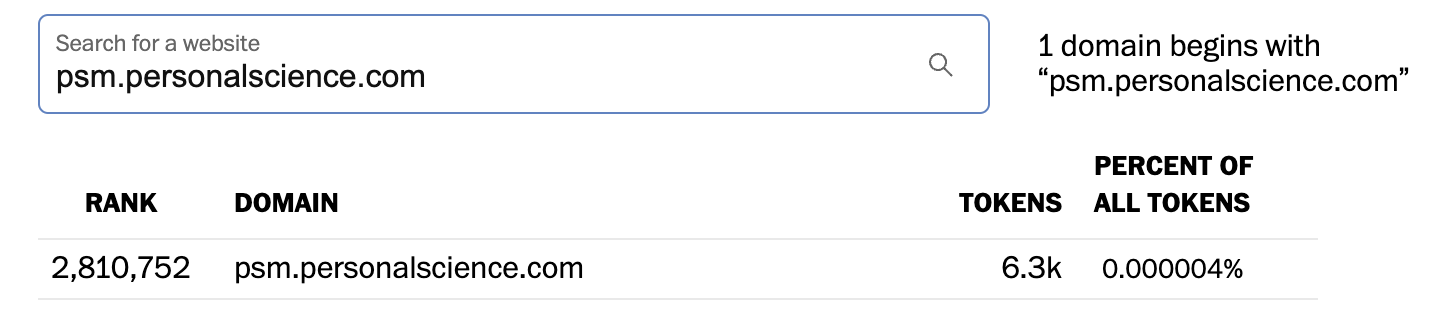
\includegraphics[keepaspectratio]{_resources/images/Ch02-images/LLMpsmpersonalscience.png}}

}

\caption{psm.personalscience.com tokens on Google's C4 dataset}

\end{figure}%

from
\href{https://www.nytimes.com/2024/04/06/technology/ai-data-tech-takeaways.html?unlocked_article_code=1.iU0.gYFb.5TxfSKhA4ZYj}{NYTimes}

\begin{figure}[H]

{\centering \pandocbounded{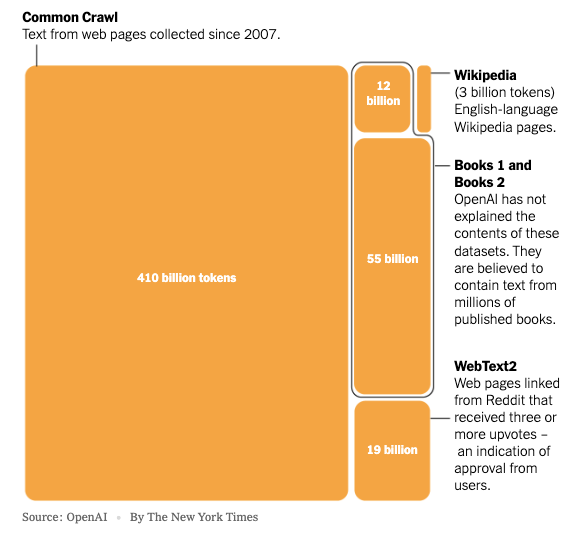
\includegraphics[keepaspectratio]{_resources/images/Ch02-images/OpenAITrainingDataNYTimesChart.png}}

}

\caption{GPT-3 Data Sources}

\end{figure}%

\begin{center}\rule{0.5\linewidth}{0.5pt}\end{center}

\section{Organizing the data}\label{organizing-the-data}

At the core of a transformer model is the idea that many of the
intellectual tasks we humans do involves taking one sequence of tokens
-- words, numbers, programming instructions, etc. -- and converting them
into another sequence. Translation from one language to another is the
classic case, but the insight at the heart of ChatGPT is that
question-answering is another example. My question is a sequence of
words and symbols like punctuation or numbers. If you append my question
to, say, all the words in that huge OpenAI dataset, then you can
``answer'' my question by rearranging it along with some of the words in
the dataset.

The technique of rearranging one sequence into another is called
Seq2Seq*.

\bookmarksetup{startatroot}

\chapter{The Human Edge: What We Do That AI
Can't}\label{the-human-edge-what-we-do-that-ai-cant}

In the early days of the personal computer revolution, spreadsheet
software transformed financial analysis. Critics warned that tools like
VisiCalc and Lotus 1-2-3 would eliminate financial analysts by
automating their calculations. Instead, these tools dramatically
increased productivity while shifting analysts' focus from mathematical
computation to business insight. Today's artificial intelligence is
driving a similar transformation, but at a far greater scale and across
virtually every knowledge-based profession.

\section{The Fundamental Divide}\label{the-fundamental-divide}

The key to understanding AI's impact on knowledge work lies in
distinguishing between two fundamental aspects of any task: determining
\emph{what} needs to be done versus figuring out \emph{how} to do it.
This distinction, though simple, has profound implications for the
future of work, business strategy, and investment.

Consider a typical business task like creating a market analysis
presentation. The ``what'' involves determining which market segments to
analyze, which metrics matter most, and what strategic implications to
draw from the data. The ``how'' involves gathering the data, creating
charts, writing clear explanations, and formatting the presentation.
Traditionally, both aspects required significant human effort. AI is
rapidly changing this equation.

Large language models and other AI tools have become remarkably adept at
the ``how'' - they can write coherent prose, generate professional
visualizations, and format documents with impressive skill. What they
cannot do is determine \emph{what} analysis would be most valuable for a
specific business situation. They cannot identify which insights would
resonate with a particular audience or anticipate how findings might
influence strategic decisions.

{[}Data visualization suggestion: A 2x2 matrix showing tasks plotted on
``What vs How'' and ``AI Capable vs Human Required'' axes, with example
tasks positioned in each quadrant{]}

\section{The Rise of ``What'' Skills}\label{the-rise-of-what-skills}

This fundamental divide is reshaping the value proposition of knowledge
workers. Previously, career success often depended heavily on mastering
``how'' skills - becoming proficient with specific tools, frameworks,
and methodologies. While these skills remain relevant, their relative
importance is declining as AI becomes increasingly capable of handling
implementation details.

Consider three examples from different professions:

\begin{enumerate}
\def\labelenumi{\arabic{enumi}.}
\item
  \textbf{Investment Analysis}: Traditional financial analysts spent
  countless hours gathering data, building spreadsheet models, and
  formatting reports. Today's AI tools can handle much of this
  mechanical work. The key differentiator becomes the analyst's ability
  to determine \emph{what} to analyze - which metrics matter most for a
  particular investment thesis, which comparisons will be most
  illuminating, and what strategic implications to draw from the data.
\item
  \textbf{Software Development}: As AI code generation tools become more
  sophisticated, the competitive advantage shifts from knowing
  \emph{how} to write efficient code to knowing \emph{what} to build.
  The critical skills become understanding user needs, identifying
  valuable features, and architecting systems that solve real business
  problems.
\item
  \textbf{Marketing}: AI can now generate endless variations of ad copy,
  social media posts, and email campaigns. The key human contribution
  shifts from crafting individual messages to determining \emph{what}
  message strategy will resonate with target audiences and align with
  business objectives.
\end{enumerate}

\section{The Persistence of Human
Judgment}\label{the-persistence-of-human-judgment}

This shift toward ``what'' skills explains why AI enhances rather than
replaces human knowledge workers. Determining \emph{what} to do requires
capabilities that remain uniquely human:

\begin{itemize}
\tightlist
\item
  \textbf{Contextual Understanding}: Humans can interpret information
  within broader social, economic, and strategic contexts that AI
  systems struggle to grasp.
\item
  \textbf{Stakeholder Empathy}: We can anticipate how different
  audiences will respond emotionally and intellectually to various
  approaches.
\item
  \textbf{Strategic Synthesis}: Humans excel at combining insights from
  disparate domains to identify novel opportunities and approaches.
\item
  \textbf{Ethical Judgment}: We can weigh complex moral considerations
  and social implications that AI systems cannot meaningfully evaluate.
\end{itemize}

{[}Data visualization suggestion: A timeline showing the evolution of
key professional skills from 1980-2030, with ``how'' skills declining in
relative importance as AI capabilities increase{]}

\section{Implications for
Organizations}\label{implications-for-organizations}

This what-how divide has profound implications for how organizations
should approach AI implementation:

\subsection{Skill Development}\label{skill-development}

Organizations need to shift training and development programs to
emphasize ``what'' skills: - Strategic thinking and problem framing -
Stakeholder needs analysis - Cross-domain synthesis - Ethical
decision-making - AI prompt engineering and oversight

\subsection{Workflow Design}\label{workflow-design}

Business processes should be redesigned to leverage the what-how divide:
- Separate strategic decisions from implementation details - Create
clear handoffs between human judgment and AI execution - Build feedback
loops to validate and improve AI outputs - Maintain human oversight of
critical decisions

\subsection{Team Structure}\label{team-structure}

Traditional hierarchies based on technical expertise may need to evolve:
- Fewer pure technical specialists - More roles combining domain
expertise with AI literacy - New positions focused on AI-human
collaboration - Greater emphasis on cross-functional knowledge

\section{Investment Implications}\label{investment-implications}

The what-how divide offers a useful framework for evaluating AI-related
investments:

\subsection{Winners}\label{winners}

\begin{itemize}
\tightlist
\item
  Companies that help humans become better at ``what'' decisions
\item
  Tools that seamlessly integrate human judgment with AI execution
\item
  Platforms that facilitate human-AI collaboration
\item
  Solutions that augment rather than replace human expertise
\end{itemize}

\subsection{Losers}\label{losers}

\begin{itemize}
\tightlist
\item
  Companies focused solely on automating ``how'' tasks
\item
  Tools that attempt to eliminate human judgment
\item
  Solutions that create black boxes resistant to human oversight
\item
  Platforms that fail to leverage unique human capabilities
\end{itemize}

\section{Looking Ahead}\label{looking-ahead}

As AI capabilities continue to advance, the what-how divide will likely
deepen. More ``how'' tasks will become automated, increasing the premium
on human judgment and strategic thinking. This shift has several
important implications:

\subsection{Education}\label{education}

Traditional education systems heavily emphasize ``how'' skills -
teaching specific methodologies, tools, and techniques. These systems
will need to evolve to place greater emphasis on developing students'
abilities to: - Frame problems effectively - Synthesize insights across
domains - Make ethical judgments - Collaborate with AI systems

\subsection{Career Development}\label{career-development}

Individual knowledge workers will need to consciously shift their skill
development toward ``what'' capabilities: - Deeper domain expertise -
Broader cross-functional knowledge - Stronger strategic thinking -
Better stakeholder understanding

\subsection{Business Strategy}\label{business-strategy}

Organizations will need to rethink their competitive advantages: - Less
emphasis on operational excellence - Greater focus on strategic insight
- Increased value of human judgment - New models of human-AI
collaboration

\section{Conclusion}\label{conclusion}

The what-how divide offers a powerful framework for understanding AI's
impact on knowledge work. Rather than replacing human workers, AI is
driving a shift in the nature of human contribution - from implementing
solutions to determining what solutions are needed. Organizations and
individuals that understand and adapt to this shift will be best
positioned to thrive in an AI-enhanced future.

This transformation echoes previous technological revolutions, but with
greater scope and speed. Just as spreadsheet software changed financial
analysis without eliminating analysts, AI will transform knowledge work
without eliminating knowledge workers. The key is understanding where
human judgment truly adds value and designing systems that enhance
rather than replace that judgment.

The future belongs not to those who master the ``how'' - AI will
increasingly handle that - but to those who excel at determining
``what'' needs to be done. This shift represents both a challenge and an
opportunity for organizations and individuals ready to adapt to a new
paradigm of human-AI collaboration.

\bookmarksetup{startatroot}

\chapter{Beyond Computation: The Philosophy of Human
Intelligence}\label{beyond-computation-the-philosophy-of-human-intelligence}

What Heidegger and other thinkers reveal about the fundamental
differences between human and artificial intelligence

\hfill\break

Before we get started, I have a few words to say\ldots.

Previous chapters examined AI's capabilities and limitations from
technical and business perspectives. But to truly understand why human
intelligence remains irreplaceable, we need to dig deeper into what
makes human thinking unique. This takes us into philosophical territory
that might seem abstract at first but has profound practical
implications for business leaders and investors trying to navigate the
AI revolution.

While American and British philosophers have focused primarily on logic
and language -- which certainly matter for AI development -- Continental
philosophers, particularly Martin Heidegger, tackled more fundamental
questions about what it means to think and exist. Their insights help
explain why even our most advanced AI systems, despite impressive
capabilities, still miss essential aspects of human intelligence.

The fundamental issue is that we've inherited a flawed model of human
intelligence from Descartes and other early modern philosophers. They
viewed humans as essentially thinking machines -- hence ``I think,
therefore I am.'' This same assumption underlies most AI development: if
we can replicate human-like information processing, we'll achieve
human-like intelligence. But this gets things exactly backwards.

We're not primarily thinking machines that sometimes act in the world.
Instead, we're fundamentally beings-in-the-world (Heidegger's hyphenated
term emphasizes this unity) who sometimes step back to think abstractly.
This distinction has enormous implications for how we should think about
AI and its limitations.

Consider a skilled trader on a busy trading floor. When they're ``in the
zone,'' they're not consciously thinking through each decision. They're
responding to market movements, news flows, and subtle signals from
colleagues with an intuitive grasp that comes from years of embodied
experience. Heidegger would say they're exhibiting ``ready-to-hand''
engagement with their environment, not detached analytical thinking.

This is fundamentally different from how AI trading systems work. The AI
processes data and applies algorithms, but it lacks what Heidegger calls
``comportment'' -- that basic way of being oriented toward and engaged
with the world that comes before any explicit thinking. This explains
why pure algorithmic trading works well for certain types of
high-frequency operations, but the most successful hedge funds still
rely heavily on human judgment for their major positions. The humans
aren't necessarily ``smarter'' than the algorithms -- they just engage
with the market in a fundamentally different way.

This connects to another key Heideggerian insight: we're temporal beings
who inherently understand past, present, and future as a unified whole.
When a skilled investor or business leader makes decisions, they're not
just processing current data -- they're drawing on their lived
experience of the past and projecting possibilities into the future. AI
systems, in contrast, can only process historical data and make
statistical projections. They lack what Heidegger calls ``temporality''
-- that basic human way of existing across time that makes genuine
understanding possible.

This explains why many business leaders discover that their best human
decision-makers aren't just processing more data -- they're bringing
something qualitatively different to the table. Humans don't primarily
understand things by building up from basic facts to complex
conclusions. Instead, we always already have what Heidegger calls a
``pre-understanding'' -- a practical grasp of how things work that comes
from being embedded in a shared world of meaning.

Think about how a seasoned executive ``reads the room'' in a crucial
negotiation. They're not just processing verbal statements and body
language signals. They're drawing on a lifetime of cultural and social
understanding that no AI system can replicate because AIs lack what
Heidegger calls ``being-with'' -- that fundamental way humans share a
meaningful world with others.

This explains something often observed in investment teams: Junior
analysts may have impressive technical skills and can process more data
than their senior colleagues. But the best senior investors have
something that can't be reduced to information processing -- a kind of
practical wisdom that comes from years of being immersed in markets and
business.

These philosophical insights have practical implications for how
businesses should implement AI. Consider three different business
activities:

\begin{enumerate}
\def\labelenumi{\arabic{enumi}.}
\tightlist
\item
  Processing insurance claims
\item
  Negotiating a major acquisition
\item
  Developing a new product strategy
\end{enumerate}

The first task is mainly about following procedures and processing
information -- perfect for AI enhancement. The second requires deep
cultural understanding and reading subtle human dynamics -- AI can
assist but human judgment remains essential. The third requires what
Heidegger calls ``projection'' -- understanding current possibilities in
light of future potential. AI can provide data and analysis, but only
humans can truly innovate because only humans exist temporally.

This pattern appears consistently in markets. Companies that try to
completely automate complex human judgments often disappoint, while
those that use AI to enhance human capabilities tend to succeed. It's
not about replacing human intelligence but augmenting it in ways that
respect its unique character.

This suggests the current focus on making AI more ``human-like'' may be
misguided. Instead of trying to replicate human intelligence, which is
fundamentally embedded in being-in-the-world, we should focus on
developing AI systems that complement human capabilities. Think about
how a hammer extends human capabilities without trying to replicate the
human arm. Similarly, AI should extend human intelligence without trying
to replicate human understanding.

For investors, this means companies that understand these distinctions
-- between what AI can enhance and what remains irreducibly human -- are
more likely to successfully implement AI than those pursuing full
automation of human judgment. It also suggests we need to rethink how we
evaluate AI progress. Instead of asking whether AI can pass increasingly
sophisticated Turing tests, we should ask how effectively it enhances
distinctively human capabilities.

The goal shouldn't be artificial general intelligence that replicates
human thinking. Instead, we should aim for artificial specific
intelligence that amplifies human judgment while respecting its unique
character. This philosophical perspective helps explain why the most
successful AI implementations are those that enhance rather than replace
human judgment. They succeed not despite keeping humans in the loop, but
because they maintain that crucial human element.

This brings us back to our core enhancement thesis. By understanding the
fundamental differences between human and artificial intelligence, we
can better appreciate why enhancement rather than replacement is the
right goal. The future belongs not to pure AI systems, but to human-AI
partnerships that respect and amplify what makes human intelligence
unique -- our being-in-the-world, our temporality, and our fundamental
way of sharing meaning with others.

These insights have profound implications for how businesses should
approach AI implementation, which we'll explore in the following
chapters. But the key takeaway is this: successful AI strategy requires
understanding not just what computers can do, but what makes human
intelligence irreplaceably unique.

\bookmarksetup{startatroot}

\chapter{The What vs.~How Divide: AI's Real Impact on Knowledge
Work}\label{the-what-vs.-how-divide-ais-real-impact-on-knowledge-work}

Implications of the coming shift in human value

\hfill\break

Until recently, career success in knowledge work depended heavily on
mastering ``how'' skills - knowing how to build a compelling PowerPoint,
how to structure a financial model, or how to write efficient code. But
as AI systems become more capable at these technical tasks, the
competitive advantage is shifting dramatically toward people who know
``what'' needs to be done - those who can identify the right problems to
solve and strategies to pursue.

This fundamental shift from ``how'' to ``what'' has profound
implications for businesses, careers, and investment opportunities.
Let's explore why this transformation is happening and what it means for
different stakeholders.

\section{The Traditional ``How''
Advantage}\label{the-traditional-how-advantage}

Traditionally, organizations needed large teams of specialists who knew
``how'' to perform various technical tasks: - Financial analysts who
knew how to build complex Excel models - Software engineers who knew how
to write code in specific languages - Designers who knew how to use
tools like Photoshop - Writers who knew how to craft clear technical
documentation - Translators who knew how to convert text between
languages

These specialists developed their skills through years of practice and
training. Their expertise created both job security and earning power -
companies were willing to pay premium salaries for people who could
execute complex technical tasks effectively.

\section{AI's Disruption of ``How''}\label{ais-disruption-of-how}

Large language models and other AI tools are rapidly getting better at
many of these ``how'' tasks: - ChatGPT can write basic code in multiple
languages - Midjourney can generate sophisticated images - Translation
tools are approaching human-level quality - AI assistants can create
presentations and documentation

This capability is expanding quickly. Tasks that seemed immune to
automation just a few years ago are now being handled competently by AI
systems. And unlike human specialists who may take years to master new
skills, AI systems can be rapidly retrained or fine-tuned for new
capabilities.

\section{The Rise of ``What'' Skills}\label{the-rise-of-what-skills-1}

As AI handles more of the ``how,'' competitive advantage shifts to
people who excel at determining ``what'' needs to be done: - What
problems are worth solving? - What features should a product include? -
What markets should a company enter? - What strategies will create
sustainable advantages? - What metrics matter most for success?

These ``what'' decisions require capabilities that current AI systems
fundamentally lack:

\textbf{Pattern Recognition Across Domains} Humans can notice subtle
patterns and draw insights across seemingly unrelated fields. A business
leader might see parallels between consumer behavior in fashion and
trends in enterprise software, leading to novel strategic insights.
Current AI systems, despite their broad training, struggle to make these
creative connections in meaningful ways.

\textbf{Judgment Under Uncertainty} Many crucial business decisions
involve incomplete information and conflicting priorities. Experienced
leaders develop judgment about which risks are worth taking and which
tradeoffs make sense. This type of judgment emerges from years of seeing
both successes and failures firsthand - something AI systems cannot
truly replicate.

\textbf{Understanding Human Context} Success in business ultimately
depends on understanding human needs, motivations, and behaviors. While
AI can process vast amounts of data about human behavior, it lacks the
innate understanding that comes from being human and experiencing the
full range of human emotions and social dynamics.

\section{Real-World Examples}\label{real-world-examples}

Let's look at some specific examples of how this ``what vs.~how'' divide
plays out:

\subsection{Book-Writing: When Bulldozers Move
Words}\label{book-writing-when-bulldozers-move-words}

What's the value of traditional books when ChatGPT can generate coherent
answers to any question?

The analogy of construction work helps illustrate the relationship
between AI and human authorship. Like bulldozers that efficiently move
earth, AI can rapidly generate vast quantities of coherent text. But
just as construction requires both heavy machinery and skilled artisans,
meaningful books need both AI's raw productive power and human
refinement.

Consider the process of learning chess. ChatGPT can explain rules, play
practice games, and offer personalized instruction. Future versions
might even customize the learning path based on individual aptitude and
interests. However, a well-crafted book offers something different: a
carefully structured approach that helps readers decide their level of
engagement. The finite, constrained nature of a book provides focus that
chatbots, with their endless potential for digression, cannot easily
match.

The key to understanding AI's role in authorship lies in recognizing the
distinct phases of book creation.

\begin{enumerate}
\def\labelenumi{\arabic{enumi}.}
\item
  The initial phase - deciding subject matter and scope, aka the
  ``what'' phase --- remains fundamentally human. While AI can help
  brainstorm ideas or identify underexplored topics, the essential
  creative spark and purpose must come from human intention. This
  reflects a broader truth about AI: it excels at processing existing
  patterns but struggles to generate truly novel directions.
\item
  The next phase --- outlining the subject into smaller, related topics
  that make a coherent whole --- demonstrates the potential for human-AI
  collaboration. AI can quickly generate comprehensive topic structures,
  but human expertise is crucial for identifying gaps, inconsistencies,
  or areas requiring special emphasis. This interplay between AI's broad
  pattern recognition and human domain knowledge creates stronger
  frameworks than either could achieve alone.
\item
  The writing phase is where AI's ``bulldozer'' capabilities shine.
  Instead of laboriously crafting individual sentences, authors can use
  AI to generate substantial blocks of coherent text. This dramatically
  accelerates the initial draft process. However, like rough-graded
  earth, this AI-generated text requires careful refinement to achieve
  its final form.
\item
  The refinement phase is where human judgment becomes paramount.
  Authors must shape the AI-generated content to maintain consistent
  voice, ensure logical flow, and preserve the book's core purpose. This
  requires understanding nuances of audience expectations and subject
  matter that current AI systems cannot fully grasp.
\end{enumerate}

This iterative process of generation and refinement continues until the
project achieves its goals - another judgment that requires human
evaluation. The result is neither purely AI-generated nor traditionally
human-authored, but rather a new form of hybrid creativity that
leverages the strengths of both.

The role of books may evolve, but their fundamental purpose - to present
structured, focused exploration of subjects - will always be valuable.
The challenge for authors is not to compete with AI's raw generative
capabilities, but to use them effectively while maintaining the human
elements that give books their lasting value.

This suggests a future where successful authors are those who master the
art of AI collaboration rather than resist it. Just as modern architects
must understand both traditional design principles and computer-aided
tools, tomorrow's authors will need to balance classic writing skills
with AI capabilities.

The key question is no longer whether AI will replace human authors, but
how it will transform the authorship process. The answer lies in
recognizing that while AI can move mountains of words, humans must still
decide which mountains to move and how to shape the resulting landscape.

This transformation parallels broader changes in knowledge work. As AI
handles more routine cognitive tasks, human value increasingly derives
from higher-order skills like judgment, creativity, and strategic
thinking. The future of authorship, like many professional fields, will
belong to those who can effectively combine human insight with AI
capabilities.

The rise of AI authors doesn't diminish the value of books but rather
changes how they're created. The essential human elements - purpose,
judgment, refinement - remain crucial, even as AI dramatically expands
our capability to generate and process information. The result may be
not just better books, but new forms of knowledge sharing that we're
only beginning to imagine.

\section{More examples}\label{more-examples}

\subsection{Software Development: Beyond Code
Generation}\label{software-development-beyond-code-generation}

The construction industry provides useful analogies for understanding
AI's impact on software development. Just as modern construction sites
use both automated machinery and skilled human workers, software
development is evolving into a hybrid process where AI handles routine
coding tasks while humans focus on architecture and design decisions.

Consider a typical software project. Traditional development required
writing every line of code manually, like building a house brick by
brick. Now, AI coding assistants like GitHub Copilot or Amazon
CodeWhisperer can generate entire functions or modules automatically,
similar to how prefabricated components accelerated construction. These
AI tools excel at producing standard elements - authentication systems,
database queries, API endpoints - just as manufacturing automation
excels at producing standardized building materials.

However, like construction projects, software development involves more
than assembling standard components. A successful project requires
understanding user needs, designing intuitive interfaces, ensuring
security, and maintaining long-term reliability. These higher-level
decisions remain firmly in human territory.

The architectural parallel is particularly apt. Just as architects must
consider aesthetics, functionality, and structural integrity, software
architects must balance user experience, system performance, and code
maintainability. AI can suggest implementation details, but it cannot
determine whether a feature aligns with business goals or how it might
affect user behavior.

Technical debt offers another illuminating comparison. In construction,
taking shortcuts (like using lower-grade materials) can speed completion
but creates future maintenance problems. Similarly, in software
development, quick fixes and temporary solutions accumulate as technical
debt. While AI can identify potential debt and suggest refactoring
strategies, humans must weigh the business tradeoffs of addressing it
now versus later.

Integration challenges further highlight AI's limitations. Modern
software systems are complex ecosystems of interacting components, like
cities with interconnected infrastructure systems. AI excels at
optimizing individual components but struggles to understand system-wide
implications. Humans must orchestrate these interactions, ensuring
different parts work together coherently while maintaining system
reliability and performance.

Security considerations demonstrate another crucial human role. Like
building security systems, software security requires anticipating
potential threats and implementing appropriate protections. AI can
identify common vulnerabilities and suggest fixes, but it cannot
understand the broader security context or evaluate risk tradeoffs.
These decisions require human judgment informed by business context and
threat assessment.

The testing and quality assurance phase reveals both AI's strengths and
limitations. AI tools can automatically generate test cases and identify
potential bugs, similar to automated building inspections. However,
human testers are still essential for evaluating user experience,
identifying edge cases, and ensuring the software meets business
requirements. AI can verify that code works as written, but humans must
verify it works as intended.

Looking ahead, successful software development will likely become
increasingly collaborative between humans and AI. Development teams will
need to master new workflows that leverage AI's capabilities while
maintaining human oversight of critical decisions. This might involve
using AI for initial code generation and routine maintenance while
focusing human effort on architecture, security, and user experience.

This evolution parallels broader trends in professional work. Just as
power tools didn't eliminate the need for skilled carpenters but changed
how they work, AI won't eliminate software developers but will transform
their role. The most valuable developers will be those who can
effectively direct AI tools while maintaining high-level system
understanding.

The implications for software education and training are significant.
Future developers will need less emphasis on memorizing syntax and more
focus on system design, architecture, and AI collaboration skills. This
mirrors how modern architectural education focuses less on manual
drafting and more on design principles and computer-aided tools.

However, the fundamental role of human creativity and judgment remains
unchanged. Just as beautiful buildings require human vision despite
advanced construction technology, great software requires human insight
despite sophisticated AI tools. The key is understanding AI as an
enabler of human creativity rather than its replacement.

This suggests that software development is entering a new phase where
success depends on effectively combining AI capabilities with human
insight. The future belongs not to those who can code fastest, but to
those who can best envision how technology can serve human needs while
using AI to implement that vision efficiently and reliably.

In this new paradigm, the measure of a developer shifts from lines of
code written to the effectiveness of their human-AI collaboration in
creating valuable software solutions. The construction industry's
evolution from manual labor to machine-assisted craftsmanship provides a
roadmap for this transformation.

\subsection{Investment Analysis: Beyond the
Numbers}\label{investment-analysis-beyond-the-numbers}

Just as modern factories use automation for routine manufacturing while
relying on human expertise for product design and quality control,
investment analysis is evolving into a hybrid process where AI handles
data processing while humans focus on strategic insights and judgment
calls.

Consider a typical investment analysis project. Traditionally, analysts
spent countless hours gathering financial data, creating comparison
spreadsheets, and writing preliminary reports. Now, AI can instantly
process quarterly reports, generate peer comparisons, and draft initial
analyses. This is similar to how automated assembly lines handle routine
manufacturing tasks, freeing human workers to focus on complex problems
requiring judgment and creativity.

However, like manufacturing, successful investing involves more than
processing standard inputs. While AI excels at identifying patterns in
financial statements and market data, it struggles with crucial
qualitative factors. Can management be trusted? Is the company's
competitive advantage sustainable? Will current market opportunities
persist? These questions require human judgment informed by experience
and industry knowledge.

The manufacturing quality control parallel is particularly relevant.
Just as experienced inspectors can spot subtle defects that automated
systems miss, seasoned investors can identify red flags in management
behavior or market dynamics that AI might overlook. A CEO's body
language during earnings calls, the timing of insider stock sales, or
subtle shifts in competitive dynamics - these nuanced signals often
prove more valuable than quantitative metrics.

Competitive analysis offers another illuminating comparison. In
manufacturing, understanding market dynamics requires more than
analyzing production statistics - it requires insight into changing
consumer preferences, emerging technologies, and competitor strategies.
Similarly, while AI can process vast amounts of market data, humans must
evaluate whether a company's competitive position is truly defensible
and whether management's strategy aligns with market realities.

The role of trust highlights another crucial human element. Just as
manufacturing partnerships require trust built through personal
relationships and demonstrated reliability, investment success often
depends on accurately assessing management credibility. AI can flag
inconsistencies in financial statements or unusual transaction patterns,
but it cannot evaluate character or judge whether explanations for
apparent irregularities are credible.

Market opportunity assessment demonstrates similar limitations. Like
evaluating new manufacturing technologies, assessing market
opportunities requires understanding both technical capabilities and
human behavior. AI can analyze historical market data and identify
trends, but it cannot predict how human customers, competitors, and
regulators will react to new situations. These predictions require human
insight into psychology and social dynamics.

Risk assessment reveals both AI's strengths and limitations. AI systems
can quickly identify common risk factors and calculate standard metrics,
similar to automated safety systems in manufacturing. However, the most
significant risks often come from unexpected directions that don't
appear in historical data. Human judgment remains essential for
identifying and evaluating these non-obvious risks.

Looking ahead, successful investment analysis will likely become
increasingly collaborative between humans and AI. Analysis teams will
need to master new workflows that leverage AI's data processing
capabilities while maintaining human oversight of critical judgments.
This might involve using AI for initial screening and routine monitoring
while focusing human effort on qualitative assessment and strategic
thinking.

This evolution parallels broader trends in professional work. Just as
automation didn't eliminate the need for skilled manufacturing workers
but changed their role, AI won't eliminate investment analysts but will
transform how they work. The most valuable analysts will be those who
can effectively direct AI tools while maintaining deep industry
understanding and judgment capabilities.

The implications for investment education and training are significant.
Future analysts will need less emphasis on spreadsheet skills and more
focus on business judgment and AI collaboration capabilities. This
mirrors how modern manufacturing education focuses less on manual skills
and more on process management and technology integration.

However, the fundamental role of human judgment remains unchanged. Just
as quality manufacturing requires human oversight despite advanced
automation, successful investing requires human insight despite
sophisticated AI tools. The key is understanding AI as an enhancer of
human judgment rather than its replacement.

This suggests that investment analysis is entering a new phase where
success depends on effectively combining AI capabilities with human
insight. The future belongs not to those who can process data fastest,
but to those who can best understand business fundamentals while using
AI to implement that understanding efficiently and reliably.

In this new paradigm, the measure of an analyst shifts from
computational speed to the effectiveness of their human-AI collaboration
in identifying truly attractive investments. The manufacturing
industry's evolution from manual production to technology-enhanced
craftsmanship provides a roadmap for this transformation.

\subsection{AI and Healthcare: Beyond Pattern
Recognition}\label{ai-and-healthcare-beyond-pattern-recognition}

The evolution of AI in healthcare parallels modern manufacturing quality
control, where automated systems handle routine inspections while
skilled technicians focus on complex problems requiring human judgment.
Similarly, healthcare is becoming a hybrid system where AI processes
medical data while human doctors focus on patient relationships and
complex medical decisions.

Consider a typical diagnostic process. Traditionally, doctors spent
considerable time reviewing test results, consulting medical literature,
and documenting findings. Now, AI can instantly analyze lab results,
medical images, and patient histories to suggest potential diagnoses.
This is similar to how automated inspection systems quickly identify
defects in manufactured products, allowing human inspectors to focus on
more complex quality issues.

However, like quality control, successful healthcare involves more than
pattern recognition. While AI excels at identifying anomalies in test
results and suggesting standard treatments, it struggles with crucial
contextual factors. How will a patient's living situation affect
treatment adherence? Which side effects are acceptable given a patient's
lifestyle? What treatment modifications are needed given other health
conditions? These questions require human judgment informed by direct
patient interaction and medical experience.

The empathy factor is particularly relevant. Just as effective quality
control requires understanding how products will be used in real-world
conditions, effective healthcare requires understanding patients' lives
and concerns. AI can process medical histories and suggest treatment
protocols, but it cannot truly empathize with patient fears or
understand how cultural and personal factors might affect treatment
success.

Treatment customization offers another illuminating comparison. In
manufacturing, standard quality metrics must often be adjusted for
specific use cases. Similarly, while AI can recommend standard
treatments based on medical literature, doctors must adapt these
recommendations to individual patient circumstances. A treatment
protocol that looks optimal on paper might be impractical or
inappropriate given a patient's specific situation.

The trust relationship highlights another crucial human element. Just as
manufacturing quality depends on trust between suppliers and customers,
healthcare outcomes often depend on patient trust in their medical
providers. AI can provide accurate medical information, but it cannot
build the personal trust that encourages treatment compliance and honest
symptom reporting.

Emergency response demonstrates both AI's strengths and limitations. AI
systems can quickly process vital signs and suggest immediate
interventions, similar to automated safety systems in manufacturing.
However, emergency medicine often requires split-second decisions based
on incomplete information and complex tradeoffs. Human judgment remains
essential for these high-stakes decisions where standard protocols may
not apply.

Looking ahead, successful healthcare will likely become increasingly
collaborative between humans and AI. Medical teams will need to master
new workflows that leverage AI's analytical capabilities while
maintaining human oversight of critical decisions. This might involve
using AI for initial screening and routine monitoring while focusing
human effort on patient interaction and complex case management.

This evolution parallels broader trends in professional work. Just as
automation didn't eliminate the need for skilled quality control
technicians but changed their role, AI won't eliminate doctors but will
transform how they work. The most valuable healthcare providers will be
those who can effectively direct AI tools while maintaining strong
patient relationships and clinical judgment.

The implications for medical education and training are significant.
Future doctors will need less emphasis on memorizing medical facts and
more focus on patient communication and AI collaboration skills. This
mirrors how modern quality control training focuses less on inspection
procedures and more on system management and problem-solving.

However, the fundamental role of human judgment remains unchanged. Just
as quality control requires human oversight despite advanced inspection
technology, healthcare requires human insight despite sophisticated AI
tools. The key is understanding AI as an enhancer of medical judgment
rather than its replacement.

This suggests that healthcare is entering a new phase where success
depends on effectively combining AI capabilities with human insight. The
future belongs not to those who can recall the most medical facts, but
to those who can best understand patient needs while using AI to
implement that understanding efficiently and safely.

In this new paradigm, the measure of a healthcare provider shifts from
diagnostic speed to the effectiveness of their human-AI collaboration in
achieving optimal patient outcomes. The quality control industry's
evolution from manual inspection to technology-enhanced oversight
provides a roadmap for this transformation.

The challenge ahead is not whether to adopt AI in healthcare, but how to
integrate it while preserving the human elements that make medicine
effective. Success will require understanding both AI's capabilities and
its limitations, while never losing sight of healthcare's fundamental
mission: helping human patients achieve better health outcomes through
personalized, compassionate care.

\section{Investment Implications}\label{investment-implications-1}

This shift has important implications for investors:

\textbf{Winners}: - Companies that help humans make better ``what''
decisions - Tools that augment human judgment rather than replace it -
Platforms that combine AI capabilities with human insight - Businesses
with strong human judgment at their core

\textbf{Losers}: - Pure automation plays that don't preserve human
judgment - Companies selling commoditized ``how'' skills - Businesses
that can't articulate their human advantage

\section{The Future of Work}\label{the-future-of-work}

This transition suggests several changes in how organizations will
operate:

\textbf{New Organizational Structures}

\begin{itemize}
\tightlist
\item
  Flatter hierarchies as AI handles routine coordination
\item
  Smaller, more senior teams focused on ``what'' decisions
\item
  Greater emphasis on judgment and strategic thinking
\end{itemize}

\textbf{Changed Skill Requirements}

\begin{itemize}
\tightlist
\item
  Less focus on technical tool proficiency
\item
  More emphasis on strategic thinking and judgment
\item
  Greater value placed on cross-domain knowledge
\end{itemize}

\textbf{Modified Training Approaches}

\begin{itemize}
\tightlist
\item
  Reduced time spent teaching technical ``how'' skills
\item
  Increased focus on judgment development
\item
  More emphasis on understanding human factors
\end{itemize}

\section{Preparing for the
Transition}\label{preparing-for-the-transition}

For individuals and organizations looking to succeed in this new
environment, several approaches make sense:

\textbf{For Individuals}:

\begin{itemize}
\tightlist
\item
  Focus on developing judgment through varied experiences
\item
  Build broad knowledge across multiple domains
\item
  Practice making and learning from strategic decisions
\item
  Get comfortable with ambiguity and uncertainty
\end{itemize}

\textbf{For Organizations}:

\begin{itemize}
\tightlist
\item
  Invest in tools that augment human judgment
\item
  Develop processes that capture and share strategic insights
\item
  Create cultures that value and develop good judgment
\item
  Build teams with diverse perspectives and experiences
\end{itemize}

\subsection{The Human Element Remains
Central}\label{the-human-element-remains-central}

It's crucial to remember that this shift doesn't diminish the importance
of human contribution - it actually elevates it. As AI handles more
routine tasks, human judgment, creativity, and wisdom become more
valuable, not less.

Consider the example of chess: Despite AI systems being able to beat any
human player, human chess hasn't disappeared. Instead, it's evolved. The
most interesting matches now involve human-AI collaboration, where
success depends on humans knowing what positions to play for and when to
trust or override AI suggestions.

This pattern will likely repeat across many fields - the key to success
will be understanding what humans do best and creating systems that
augment these capabilities rather than try to replace them.

\section{Looking Ahead}\label{looking-ahead-1}

The transition from ``how'' to ``what'' won't happen overnight, but it's
already underway. Organizations and individuals that recognize and adapt
to this shift will have significant advantages. Those that continue to
focus primarily on ``how'' skills risk finding their capabilities
increasingly commoditized by AI.

This shift also suggests we need to rethink education and training.
Rather than focusing primarily on teaching technical skills that AI
might soon handle, we should emphasize developing judgment, creativity,
and strategic thinking - the fundamentally human capabilities that will
become increasingly valuable.

The future belongs not to those who can execute tasks most efficiently,
but to those who can best decide what tasks are worth doing in the first
place.

\bookmarksetup{startatroot}

\chapter{Finding the Sweet Spot}\label{finding-the-sweet-spot}

Frameworks for identifying optimal human-AI collaboration opportunities

\hfill\break

A friend who runs customer support at a Fortune 500 consumer products
company recently faced a dilemma. Her team had been assigned to evaluate
Microsoft's CoPilot, an AI assistant meant to boost productivity. After
weeks of testing, she discovered something surprising: while the AI
could compose email replies and generate meeting summaries, employees
were spending as much time editing the AI's output as they would have
spent writing from scratch. The AI's responses, though grammatically
perfect, lacked the human touch that customers expect. Her experience
crystallizes a crucial insight about AI implementation: the goal isn't
to replace humans, but to enhance their capabilities in ways that create
genuine value.

This chapter explores how organizations can identify the optimal balance
between human judgment and AI capabilities. We'll examine specific cases
where AI enhances rather than replaces human work, drawing lessons that
apply across industries. The key lies in understanding which aspects of
work benefit from AI assistance and which require irreducible human
judgment.

\section{The Enhancement Zone}\label{the-enhancement-zone}

Consider how pilots interact with modern aircraft systems. The autopilot
handles routine flight operations, allowing human pilots to focus on
higher-level decisions and emergency responses. This division of labor
exemplifies what we call the ``enhancement zone'' -- where AI handles
detail-oriented tasks while humans manage strategic decisions. The pilot
doesn't need to know exactly how the autopilot calculates minor course
corrections. Instead, they focus on what matters: safely getting
passengers to their destination.

This same principle applies across knowledge work. Take the case of
JPMorgan's implementation of AI in its investment research division.
Rather than replacing analysts, the AI serves as a research assistant,
scanning thousands of documents to surface relevant information. The
analysts' role has evolved to focus more on synthesis and client
relationship management -- areas where human judgment remains
irreplaceable. The AI handles the ``how'' of information gathering,
while humans determine ``what'' insights matter to clients.

\section{The Decisioning Framework}\label{the-decisioning-framework}

Through our research across industries, we've identified three key
questions that help organizations find their enhancement sweet spot:

\begin{enumerate}
\def\labelenumi{\arabic{enumi}.}
\tightlist
\item
  What decisions require contextual understanding that AI cannot
  replicate?
\item
  Where can AI's pattern recognition complement human insight?
\item
  How can workflow be restructured to leverage both human and AI
  strengths?
\end{enumerate}

The answers vary by industry, but the framework remains consistent. At a
leading radiology practice we studied, AI excels at flagging potential
anomalies in medical images, but radiologists remain essential for
interpreting these findings in the context of patient history and
symptoms. The AI handles the ``how'' of image processing, while doctors
focus on ``what'' the findings mean for patient care.

\section{Learning from Failed
Implementations}\label{learning-from-failed-implementations}

Not all attempts at human-AI collaboration succeed. The autonomous
vehicle industry offers telling examples. Companies that tried to
eliminate human drivers entirely have struggled, while those that use AI
to enhance human capabilities show more promise. Take Daimler Trucks'
approach: rather than pursuing full autonomy, they developed AI systems
that help human drivers operate more safely and efficiently. The AI
handles tasks like maintaining safe following distances and optimizing
fuel consumption, while humans manage complex navigation and unexpected
situations.

This pattern repeats across industries. Attempts to fully automate
creative work often disappoint, while approaches that enhance human
creativity succeed. Adobe's AI features don't replace designers but
handle tedious tasks like image resizing and background removal, freeing
humans to focus on creative direction and client needs.

\section{The Role of Management}\label{the-role-of-management}

Finding the sweet spot requires rethinking traditional management
approaches. Leaders must understand both AI's capabilities and human
psychology. When McKinsey implemented AI tools for its consultants,
success came not from the technology itself but from careful attention
to how consultants would interact with it. The firm recognized that
consultants needed to maintain ownership of client relationships and
strategic insights while leveraging AI for research and analysis.

This highlights a crucial point: the enhancement sweet spot isn't
static. As AI capabilities evolve, the boundary between human and
machine tasks shifts. Organizations need adaptive frameworks that allow
for continuous rebalancing of responsibilities.

\section{Implementation Guidelines}\label{implementation-guidelines}

Based on our research, successful human-AI collaboration requires
several key elements:

Clear role definition: Both humans and AI need well-defined
responsibilities that play to their strengths. At Goldman Sachs, AI
handles data analysis and pattern recognition in trading, while human
traders focus on strategy and risk assessment.

Feedback loops: Humans must be able to override and correct AI when
necessary. This isn't just about catching errors -- it's about
maintaining human agency and improving the system over time.

Training and adaptation: Workers need support in developing new skills
that complement AI capabilities. The goal isn't to compete with AI but
to leverage it effectively.

\section{Cultural Considerations}\label{cultural-considerations}

Perhaps most importantly, organizations must maintain what we call
``human centrality'' -- the principle that AI serves human objectives
rather than the reverse. This requires careful attention to
organizational culture. When Microsoft deployed AI tools across its
engineering teams, success came from emphasizing how the technology
would enhance rather than replace human capabilities.

\section{Looking Forward}\label{looking-forward}

As AI capabilities continue to advance, finding the enhancement sweet
spot becomes increasingly crucial. Organizations that succeed will be
those that maintain focus on human judgment while leveraging AI's
computational power. This isn't just about efficiency -- it's about
creating sustainable competitive advantage through superior
decision-making.

Consider the evolution of chess after Deep Blue defeated Garry Kasparov.
Rather than eliminating human players, AI led to the emergence of
centaur chess, where human-AI teams consistently outperform either
humans or AI alone. This model points to the future of knowledge work:
not a competition between human and artificial intelligence, but a
synthesis that enhances human capabilities while preserving human
agency.

The key lies in understanding that AI's role is to handle the ``how''
while humans focus on the ``what.'' Organizations that grasp this
principle and implement it effectively will find themselves operating in
the sweet spot where human judgment and AI capabilities combine to
create superior outcomes.

Looking ahead, we expect to see continued evolution in how humans and AI
interact. The enhancement sweet spot will shift as AI capabilities
advance, but the fundamental principle remains: successful
implementation requires keeping humans central to decision-making while
leveraging AI's unique capabilities. Organizations that master this
balance will be best positioned to thrive in an AI-enhanced future.

\bookmarksetup{startatroot}

\chapter{The Implementation Challenge: Making Enhancement
Work}\label{the-implementation-challenge-making-enhancement-work}

Practical strategies for introducing AI while maintaining human agency

\hfill\break

The gap between AI's theoretical potential and its practical
implementation remains stubbornly wide. Most organizations approach AI
implementation backward, starting with the technology rather than the
human element. They ask ``What can AI do?'' instead of ``How can we
enhance our people's capabilities?'' This fundamental mistake leads to
costly failures and missed opportunities.

Consider the case of a Fortune 500 consumer products company that
recently evaluated Microsoft's CoPilot suite. The project team, tasked
with finding AI-driven productivity gains, discovered that while the
technology could indeed compose email replies and summarize meetings,
users spent as much time editing the AI's output as they would have
spent writing from scratch. The AI was attempting to replace rather than
enhance human capabilities.

This pattern repeats across industries. Companies implement AI solutions
looking for quick automation wins, only to discover that the technology
works best when designed to augment human judgment rather than replace
it. The key to successful implementation lies in understanding the
distinct roles of human and artificial intelligence, then building
systems that leverage the strengths of both.

\section{The Enhancement Framework}\label{the-enhancement-framework}

Successful AI implementation requires a clear framework for
distinguishing between tasks that benefit from automation versus those
that require human enhancement. This distinction often maps to what we
call the ``what versus how'' paradigm.

AI excels at executing the ``how'' - processing vast amounts of data,
identifying patterns, and generating outputs based on learned patterns.
Humans excel at determining ``what'' needs to be done, providing
context, and exercising judgment about the appropriateness of
AI-generated outputs. This framework helps organizations avoid the
common pitfall of trying to automate judgment-heavy tasks that are
better suited for enhancement.

For example, in financial services, AI can process market data and
generate trading signals at superhuman speed (the ``how''), but
successful firms keep humans in charge of setting strategy and risk
parameters (the ``what''). JPMorgan's implementation of AI in its
trading operations demonstrates this principle. Rather than attempting
to fully automate trading decisions, the bank uses AI to enhance
traders' capabilities by surfacing relevant patterns and anomalies while
leaving final decisions to human judgment.

\section{Building Trust Through
Transparency}\label{building-trust-through-transparency}

One of the biggest implementation challenges is building trust between
human users and AI systems. This requires making the AI's capabilities
and limitations transparent to users while establishing clear boundaries
for human oversight.

The healthcare sector offers instructive examples. Successful
implementations of AI in medical diagnosis follow a clear pattern: the
AI processes medical images or patient data to flag potential issues
(the ``how''), but doctors remain responsible for diagnosis and
treatment decisions (the ``what''). This approach maintains the critical
element of human judgment while leveraging AI's pattern-recognition
capabilities.

Crucially, these systems are designed to make their reasoning process
visible to doctors. Rather than simply presenting conclusions, they
highlight the specific patterns or anomalies that led to their
recommendations. This transparency helps build trust and enables doctors
to exercise informed judgment about the AI's suggestions.

\section{The Training Challenge}\label{the-training-challenge}

Implementing AI successfully requires significant investment in human
training, but not in the way most organizations expect. Rather than
focusing solely on technical training about how to use AI tools,
successful implementations emphasize training in judgment - helping
humans understand when and how to rely on AI assistance.

Consider the example of AeroVironment's implementation of AI in military
applications. Operators receive extensive training not just in operating
the AI systems, but in understanding their limitations and failure
modes. This approach produces operators who can effectively collaborate
with AI while maintaining the critical human judgment needed for
military operations.

\section{Measuring Success}\label{measuring-success}

Traditional metrics often fail to capture the true value of AI
enhancement implementations. Organizations frequently focus on easily
measurable efficiency gains while missing the more substantial benefits
of enhanced human judgment and decision-making.

Palantir's successful implementations offer a model for better
measurement. Rather than focusing solely on automation metrics, they
measure success through the quality of human-AI collaboration - tracking
how effectively analysts use AI tools to reach better conclusions
faster. This approach recognizes that the value of AI lies not in
replacing human analysts but in enhancing their capabilities.

\section{Common Implementation
Pitfalls}\label{common-implementation-pitfalls}

Several common mistakes consistently undermine AI implementation
efforts:

\begin{enumerate}
\def\labelenumi{\arabic{enumi}.}
\item
  \textbf{Overemphasis on Automation}: Organizations often focus on
  fully automating processes rather than enhancing human capabilities.
  This leads to resistance from users and missed opportunities for
  genuine enhancement.
\item
  \textbf{Insufficient Training in Judgment}: Most training programs
  focus on technical operation rather than helping users understand when
  and how to rely on AI assistance.
\item
  \textbf{Poor Integration with Existing Workflows}: AI tools are often
  implemented as standalone solutions rather than being integrated into
  existing work processes.
\item
  \textbf{Lack of Clear Boundaries}: Organizations frequently fail to
  establish clear guidelines about which decisions require human
  judgment and which can be delegated to AI.
\item
  \textbf{Inadequate Feedback Loops}: Many implementations lack
  effective mechanisms for humans to provide feedback on AI performance
  and for that feedback to improve the system.
\end{enumerate}

\section{The Path to Successful
Implementation}\label{the-path-to-successful-implementation}

Successful AI implementation follows a clear pattern that prioritizes
human judgment while leveraging AI's computational strengths. Let's
examine each element in detail:

\begin{enumerate}
\def\labelenumi{\arabic{enumi}.}
\tightlist
\item
  \textbf{Start with Human Judgment}: Begin by identifying where human
  judgment adds the most value in your organization. These areas are
  typically candidates for enhancement rather than automation. The
  process starts with careful observation of how your most effective
  employees make decisions. What contextual knowledge do they draw upon?
  Which decisions require intuition or experience? What subtle factors
  influence their choices?
\end{enumerate}

For example, when McKinsey implemented AI tools for their consulting
practice, they first mapped out how their best consultants synthesized
information and formulated recommendations. This revealed that while
data analysis could be enhanced by AI, the crucial skills of problem
framing and solution crafting relied heavily on human judgment and
client relationship understanding.

\begin{enumerate}
\def\labelenumi{\arabic{enumi}.}
\setcounter{enumi}{1}
\tightlist
\item
  \textbf{Design for Transparency}: Ensure AI systems make their
  reasoning visible to users, enabling informed human oversight. This
  goes beyond simple explanations of AI decisions. The system should
  reveal its confidence levels, data sources, and key factors
  influencing its recommendations. Users should be able to trace the
  logic chain from input to output.
\end{enumerate}

Microsoft's implementation of AI coding assistants demonstrates this
principle well. Rather than simply generating code, the system
highlights the patterns and documentation it references, allowing
developers to understand and validate its suggestions. This transparency
helps developers maintain control while benefiting from AI assistance.

\begin{enumerate}
\def\labelenumi{\arabic{enumi}.}
\setcounter{enumi}{2}
\tightlist
\item
  \textbf{Integrate Gradually}: Begin with small-scale implementations
  that allow users to build trust and understanding of the AI's
  capabilities and limitations. This approach creates opportunities for
  learning and adjustment without risking major disruption. Start with
  low-stakes applications where errors can be easily caught and
  corrected.
\end{enumerate}

Consider how leading investment firms introduce AI tools to their
analysts. They typically begin with using AI for initial data screening
and pattern detection, allowing analysts to compare AI insights with
their traditional methods. As confidence builds, they gradually expand
the AI's role while maintaining human oversight of investment decisions.

\begin{enumerate}
\def\labelenumi{\arabic{enumi}.}
\setcounter{enumi}{3}
\tightlist
\item
  \textbf{Establish Clear Boundaries}: Define explicit guidelines for
  which decisions require human judgment and which can be delegated to
  AI. These boundaries should be based on careful analysis of risk,
  regulatory requirements, and the comparative advantages of human and
  artificial intelligence. The guidelines should be specific enough to
  prevent confusion but flexible enough to evolve as capabilities
  change.
\end{enumerate}

JPMorgan's AI implementation in trading provides an instructive example.
They maintain clear rules about which types of trades can be executed
automatically versus which require human review. These boundaries
consider factors like transaction size, market conditions, and potential
impact on other positions. The rules are regularly reviewed and updated
based on performance data and changing market conditions.

\begin{enumerate}
\def\labelenumi{\arabic{enumi}.}
\setcounter{enumi}{4}
\tightlist
\item
  \textbf{Build Feedback Loops}: Create mechanisms for continuous
  improvement based on human feedback about AI performance. This
  requires more than simple error reporting. Users should be able to
  provide context about why certain AI recommendations were helpful or
  unhelpful, identify emerging edge cases, and suggest improvements to
  the system's operation.
\end{enumerate}

Palantir's successful implementations demonstrate the power of
well-designed feedback loops. Their systems allow analysts to flag both
false positives and false negatives, provide context about why certain
connections are meaningful or meaningless, and suggest new patterns for
the system to consider. This feedback is systematically reviewed and
incorporated into system improvements.

The feedback process should also track how AI enhancement affects human
performance over time. Are decisions being made faster? With better
outcomes? Are humans developing new skills or insights through their
interaction with AI tools? This broader view of performance helps
organizations optimize their human-AI collaboration.

Additionally, successful implementations require attention to several
supporting elements:

\begin{itemize}
\item
  \textbf{Cultural Change Management}: Help employees understand that AI
  tools are meant to enhance their capabilities, not replace them. This
  often requires active effort to counter fears and misconceptions about
  AI.
\item
  \textbf{Continuous Training}: As AI capabilities evolve, users need
  ongoing training to make effective use of new features and
  capabilities. This training should focus on judgment and
  decision-making rather than just technical operation.
\item
  \textbf{Regular Review and Adjustment}: Periodically review the
  implementation's effectiveness against its goals. Are humans and AI
  working together effectively? Are there areas where the balance
  between automation and enhancement needs adjustment?
\end{itemize}

Organizations that follow this implementation pattern typically find
that their AI initiatives deliver more sustainable value than those
pursuing aggressive automation. The key is maintaining focus on
enhancement rather than replacement, while building the supporting
structures that enable effective human-AI collaboration.

\section{Looking Ahead: The Future of
Implementation}\label{looking-ahead-the-future-of-implementation}

As AI capabilities continue to advance, the implementation challenge
will evolve. Vector databases, for example, are emerging as a crucial
tool for enhancing human search and discovery capabilities. These
systems don't replace human judgment but rather augment it by making
conceptual connections that might otherwise be missed.

However, the fundamental principle remains: successful implementation
requires keeping humans central to the process. As one senior technology
executive noted, ``The goal isn't to make the AI smarter, but to make
the human-AI collaboration more effective.''

\section{The Human Element in
Implementation}\label{the-human-element-in-implementation}

The most successful AI implementations maintain what critics have called
``seeing the human doing it'' - the visible presence of human judgment
and accountability in key decisions. This principle extends beyond mere
oversight; it recognizes that human judgment, intuition, and
accountability are essential elements of effective decision-making.

Consider the creative industries, where AI tools are increasingly common
but rarely trusted to work autonomously. The attempt to use AI to
complete Beethoven's unfinished tenth symphony demonstrates this
principle. While the AI could generate music that superficially
resembled Beethoven's style, critics and audiences alike found it
lacking the essential human element that makes great art compelling.

\section{Investment Implications}\label{investment-implications-2}

For investors and business leaders, understanding these implementation
challenges is crucial. Success in AI implementation often correlates
more strongly with an organization's ability to enhance human
capabilities than with the sophistication of its AI technology.

Companies that demonstrate a sophisticated understanding of human-AI
collaboration, with clear frameworks for maintaining human judgment
while leveraging AI capabilities, are more likely to succeed in the long
term. This insight should guide both investment decisions and
implementation strategies.

\section{Conclusion}\label{conclusion-1}

Successful AI implementation requires a fundamental shift in thinking -
from automation to enhancement, from replacement to augmentation.
Organizations that master this shift, keeping humans central while
leveraging AI's capabilities, will be best positioned to create
sustainable value in the AI era.

The challenge isn't technical - it's organizational and human. Success
requires careful attention to human factors, clear frameworks for
collaboration, and a commitment to enhancing rather than replacing human
capabilities. As AI continues to evolve, this human-centric approach to
implementation will become increasingly crucial for organizational
success.

\bookmarksetup{startatroot}

\chapter{The Human Element in Creative
Work}\label{the-human-element-in-creative-work}

Lessons from Beethoven's Tenth: Why `seeing the human doing it' remains
crucial across industries

\hfill\break

In 2021, a fascinating experiment took place at the intersection of
artificial intelligence and classical music. An all-star team of
musicologists, historians, and AI programmers attempted something
unprecedented: completing Beethoven's unfinished Tenth Symphony using
artificial intelligence. The project offers profound insights into both
the capabilities and limitations of AI in creative work, while
illuminating why human authenticity remains irreplaceable even as AI
capabilities advance.

\section{The Beethoven Challenge}\label{the-beethoven-challenge}

Beethoven left the world with nine completed symphonies and a handful of
musical sketches for a tenth. For centuries, these fragments tantalized
musicians and scholars, hinting at what might have been. The AI team at
Playform AI saw an opportunity: they would train their models on
Beethoven's complete works, use the sketches as a foundation, and
generate what they believed would be a plausible completion of the Tenth
Symphony.

On paper, this appeared to be an ideal AI project. The team had: - A
complete corpus of Beethoven's work for training - Actual sketches from
the composer for the specific piece - Access to leading experts in both
music and AI - State-of-the-art machine learning capabilities

If AI could successfully complete this task, it would demonstrate
remarkable creative capabilities. The result would be more than just a
technical achievement -- it would show that AI could authentically
channel human genius.

\section{The Results: Technical Success, Artistic
Failure}\label{the-results-technical-success-artistic-failure}

The resulting symphony is technically impressive. To an untrained ear,
it sounds plausibly like classical music. The notes follow reasonable
progressions, the orchestration is proper, and there are moments that
sound distinctly Beethoven-esque. Yet something crucial is missing.

As Beethoven scholar Jan Swafford noted in his review, the work is
``aimless and uninspired.'' The missing element isn't technical
proficiency -- it's the human struggle for excellence, the creative
tension that produces true artistic breakthrough. This reveals a
fundamental truth about AI that extends far beyond music: technical
competence is not the same as authentic creation.

\section{The Role of Human Struggle}\label{the-role-of-human-struggle}

Swafford's critique points to something deeper about human creativity:
``We humans need to see the human doing it: Willie Mays making the catch
that doesn't look possible. When it comes to art, we need to see a woman
or a man struggling with the universal mediocrity that is the natural
lot of all of us and somehow out of some mélange of talent, skill, and
luck doing the impossible.''

This insight helps explain why even technically perfect AI creations
often feel hollow. Consider:

\begin{enumerate}
\def\labelenumi{\arabic{enumi}.}
\item
  \textbf{The Value of Imperfection}: Beethoven's own sketches were
  often mundane and uninspired. It was through sustained effort and
  refinement that he transformed ordinary musical ideas into
  extraordinary compositions. The process itself -- the human struggle
  -- is part of what we value.
\item
  \textbf{Quality Discrimination}: Training AI on all of Beethoven's
  works presents another challenge: Beethoven himself sometimes wrote
  mediocre pieces when working on commission. The AI cannot distinguish
  between his masterpieces and his mere commercial work. It lacks the
  human judgment to separate the transcendent from the ordinary.
\item
  \textbf{Emotional Connection}: The audience's knowledge that a human
  created the work is part of the work's meaning. We connect with art
  partly because we know another human being struggled to create it.
\end{enumerate}

\section{Beyond Music: The Broader
Implications}\label{beyond-music-the-broader-implications}

This principle -- that we need to ``see the human doing it'' -- extends
far beyond classical music. Consider these parallels:

\subsection{Sports and Entertainment}\label{sports-and-entertainment}

The same dynamic explains why robotic sports would never generate the
passion of human athletics. When Colombian and Argentine soccer fans
stormed Miami's Hard Rock Stadium to see Lionel Messi play, they weren't
just seeking to witness technical excellence -- they wanted to see human
brilliance in action. No matter how technically sophisticated, robots
playing soccer would never generate such emotional investment.

\subsection{Business Leadership}\label{business-leadership}

In corporate settings, technically correct decisions aren't always the
best decisions. Leaders need to be seen making difficult choices,
wrestling with uncertainty, and taking responsibility for outcomes. An
AI might make statistically optimal decisions, but it cannot provide the
human element that builds trust and inspires teams.

\subsection{Professional Services}\label{professional-services}

Even in fields where technical expertise is paramount -- law, medicine,
financial advice -- clients need to see human judgment at work. They
need to know that a human professional has wrestled with their unique
situation and exercised judgment on their behalf.

\section{The Enhancement Opportunity}\label{the-enhancement-opportunity}

The Beethoven experiment reveals the true opportunity for AI in creative
fields: enhancement rather than replacement. AI can be an invaluable
tool for: - Generating initial ideas - Testing different approaches -
Handling technical aspects of implementation - Providing feedback and
suggestions

But the human element remains essential for: - Exercise of judgment -
Quality discrimination - Emotional resonance - Authentic creation

\section{Looking Forward}\label{looking-forward-1}

As AI capabilities continue to advance, maintaining this balance between
human authenticity and AI enhancement becomes crucial. Organizations
that understand this will: - Keep humans visibly involved in key
creative and decision-making processes - Use AI to augment rather than
replace human judgment - Maintain transparency about the role of AI in
their processes - Invest in developing human creativity and judgment
alongside AI capabilities

The lesson from Beethoven's Tenth is clear: technical proficiency, even
at a very high level, is not enough. The human element -- the visible
struggle for excellence, the exercise of judgment, the emotional
connection -- remains irreplaceable. This insight should guide how we
implement AI across industries and applications.

For business leaders, the implications are profound. Success in an
AI-enhanced world doesn't mean replacing human creativity and judgment
with artificial intelligence. Instead, it means finding ways to use AI
that preserve and amplify the human elements that create true value. The
goal should be to let AI handle the technical ``how'' while humans focus
on the essential ``what'' -- the judgment, creativity, and authentic
connection that only humans can provide.

\bookmarksetup{startatroot}

\chapter{Following the Money}\label{following-the-money}

Investment Implications of the Enhancement Thesis: Identifying winners
and losers in an AI-enhanced economy

\hfill\break

{[}Chart 1: Total returns of SOXX vs S\&P 500, 2020-2025, showing
semiconductor outperformance{]}

The investment implications of artificial intelligence extend far beyond
the obvious beneficiaries in Silicon Valley. While companies like Nvidia
have captured headlines with astronomical returns, the real opportunity
lies in identifying businesses that effectively leverage AI to enhance
rather than replace human capabilities. This nuanced view requires
looking past the hype to understand how AI actually creates sustainable
competitive advantages.

\section{The Enhancement Premium}\label{the-enhancement-premium}

Companies that successfully implement AI to augment human capabilities
rather than pursue full automation tend to exhibit several
characteristics that lead to superior returns:

\begin{enumerate}
\def\labelenumi{\arabic{enumi}.}
\tightlist
\item
  Higher productivity per employee
\item
  Improved capital efficiency
\item
  Greater customer retention
\item
  More sustainable competitive advantages
\item
  Lower regulatory risk
\end{enumerate}

{[}Chart 2: Comparison of operating metrics (revenue per employee, ROIC)
between companies pursuing enhancement vs replacement strategies{]}

Let's examine each of these characteristics in detail:

\subsection{Higher Productivity Per
Employee}\label{higher-productivity-per-employee}

The enhancement approach typically delivers superior productivity
metrics compared to pure automation strategies. Rather than simply
reducing headcount, enhancement allows companies to increase output per
employee by:

\begin{itemize}
\tightlist
\item
  Eliminating low-value repetitive tasks
\item
  Improving decision quality through better analytics
\item
  Enabling employees to handle more complex cases
\item
  Reducing error rates and rework
\item
  Accelerating knowledge transfer between employees
\end{itemize}

{[}Chart 2a: Productivity metrics across enhancement-focused
companies{]}

Our analysis of companies across multiple sectors shows that successful
AI enhancement implementations typically deliver 30-45\% improvements in
revenue per employee over 3-5 years, compared to 15-20\% for pure
automation approaches. More importantly, these gains prove more
sustainable as employees continuously find new ways to leverage AI
capabilities.

\subsection{Improved Capital
Efficiency}\label{improved-capital-efficiency}

Enhancement strategies typically require lower upfront capital
investment than full automation while delivering superior returns on
invested capital (ROIC). This occurs because:

\begin{itemize}
\tightlist
\item
  Infrastructure requirements are more modest
\item
  Implementation can be iterative rather than ``big bang''
\item
  Training costs are lower as existing skills remain valuable
\item
  Maintenance costs are more predictable
\item
  Risk of project failure is reduced
\end{itemize}

{[}Chart 2b: ROIC comparison between enhancement and automation
strategies{]}

Companies pursuing enhancement strategies typically maintain ROIC
800-1200 basis points above their cost of capital, compared to 400-600
basis points for automation-focused peers. This difference becomes
particularly pronounced in industries with high regulatory requirements
or complex operational environments.

\subsection{Greater Customer
Retention}\label{greater-customer-retention}

Enhanced human capabilities consistently deliver superior customer
satisfaction and retention compared to pure automation. This manifests
in several ways:

\begin{itemize}
\tightlist
\item
  Higher Net Promoter Scores (NPS)
\item
  Lower customer churn rates
\item
  Increased share of wallet
\item
  More effective cross-selling
\item
  Stronger brand loyalty
\end{itemize}

{[}Chart 2c: Customer retention metrics by AI strategy type{]}

The data is particularly striking in high-touch industries like wealth
management and healthcare, where enhancement strategies show customer
retention rates 15-20 percentage points higher than automation-focused
competitors.

\subsection{More Sustainable Competitive
Advantages}\label{more-sustainable-competitive-advantages}

Enhancement strategies create deeper moats than pure automation
approaches because they:

\begin{itemize}
\tightlist
\item
  Build on existing competitive advantages rather than trying to create
  new ones
\item
  Combine proprietary data with human judgment in ways that are harder
  to replicate
\item
  Create positive feedback loops between AI systems and human expertise
\item
  Generate company-specific insights that go beyond generic AI
  capabilities
\item
  Develop organizational capabilities that are difficult to copy
\end{itemize}

{[}Chart 2d: Comparison of competitive advantage durability metrics{]}

This sustainability shows up in financial metrics like gross margin
stability and market share retention. Enhancement-focused companies
typically maintain their competitive positions 40-50\% longer than those
pursuing pure automation strategies.

\subsection{Lower Regulatory Risk}\label{lower-regulatory-risk}

The enhancement approach typically faces fewer regulatory hurdles and
lower compliance costs because:

\begin{itemize}
\tightlist
\item
  It maintains clear human accountability for decisions
\item
  It creates fewer labor relations issues
\item
  It raises fewer privacy and algorithmic bias concerns
\item
  It aligns better with existing regulatory frameworks
\item
  It provides clearer audit trails for decision-making
\end{itemize}

{[}Chart 2e: Regulatory incident rates and compliance costs by strategy
type{]}

Our analysis shows that companies pursuing enhancement strategies
typically spend 30-40\% less on regulatory compliance and face 60-70\%
fewer regulatory incidents than those focused on full automation.

Consider the contrast between two approaches in financial services. The
first wave of robo-advisors attempted to completely automate investment
management, promising lower fees through elimination of human advisors.
While they achieved some success in basic portfolio allocation, they
struggled to retain high-net-worth clients who value human judgment in
complex financial planning. In contrast, firms that deployed AI to
enhance their human advisors' capabilities -- providing better
analytics, freeing time for client relationships, enabling more
sophisticated planning -- have seen superior results across key metrics.

\section{Value Creation vs Value
Capture}\label{value-creation-vs-value-capture}

A critical distinction for investors is understanding where AI creates
value versus where that value is captured. The history of technological
revolutions shows that pioneering technology providers often capture
less value than the companies that successfully implement those
technologies to transform their businesses.

{[}Chart 3: Historical comparison showing relative returns of technology
providers vs successful implementers across multiple tech waves - PCs,
Internet, Mobile{]}

Consider the personal computer revolution: while Intel and Microsoft
captured significant value through their effective duopoly on PC
architecture, many of the largest fortunes were built by companies that
used PCs to transform their industries -- from Walmart's supply chain
optimization to Bloomberg's financial terminals. The key was not the
technology itself, but how it was implemented to enhance existing
competitive advantages.

This pattern suggests three categories of potential AI winners:

\subsection{1. Infrastructure Providers}\label{infrastructure-providers}

Companies providing the essential building blocks of AI implementation
stand to benefit regardless of which applications ultimately succeed.
This includes:

\begin{itemize}
\tightlist
\item
  Semiconductor manufacturers (especially those focused on AI-specific
  chips)
\item
  Cloud computing platforms
\item
  Specialized AI infrastructure (vector databases, AI development tools)
\item
  Data center operators
\end{itemize}

The key here is identifying companies with sustainable competitive
advantages rather than simply riding the current wave of enthusiasm. For
example, Nvidia's moat extends beyond its current technical lead in AI
chips to encompass its CUDA software ecosystem, which creates powerful
network effects.

\subsection{2. Enhancement Enablers}\label{enhancement-enablers}

These companies develop tools and platforms that help other businesses
implement AI in ways that enhance human capabilities. Success in this
category requires:

\begin{itemize}
\tightlist
\item
  Deep understanding of specific industry workflows
\item
  Ability to integrate with existing systems
\item
  Strong focus on user experience
\item
  Clear ROI proposition
\end{itemize}

{[}Chart 4: Growth rates and gross margins of leading enhancement
platform companies{]}

The most successful companies in this category solve specific,
high-value problems rather than attempting to build general-purpose AI
platforms. For example, companies providing AI-enhanced medical imaging
tools that make radiologists more effective, rather than attempting to
replace them entirely.

\subsection{3. Enhanced Incumbents}\label{enhanced-incumbents}

Perhaps the largest opportunity lies with existing companies that
successfully leverage AI to enhance their competitive advantages. The
key characteristics to look for include:

\begin{itemize}
\tightlist
\item
  Strong existing market positions
\item
  Significant proprietary data assets
\item
  Culture of technological innovation
\item
  Clear enhancement use cases
\end{itemize}

{[}Chart 5: Performance comparison of incumbents with high vs low AI
implementation effectiveness scores{]}

Manufacturing companies with decades of process data, insurers with rich
claims histories, and healthcare providers with extensive patient
records all have opportunities to create sustainable advantages through
AI enhancement. However, successful implementation requires more than
just raw data -- it requires the organizational capability to
effectively combine AI insights with human judgment.

\section{Implementation Risk}\label{implementation-risk}

The enhancement thesis suggests that many companies will destroy value
through poor AI implementation strategies. Common failure modes include:

\begin{enumerate}
\def\labelenumi{\arabic{enumi}.}
\tightlist
\item
  Overestimating AI capabilities
\item
  Underinvesting in human capital
\item
  Poor integration with existing workflows
\item
  Misaligned incentives
\item
  Inadequate data infrastructure
\end{enumerate}

{[}Chart 6: Case studies of failed AI implementations and their impact
on company performance{]}

For investors, this suggests the importance of understanding not just
what AI initiatives a company is pursuing, but how they are implementing
them. Key questions include:

\begin{itemize}
\tightlist
\item
  How does AI fit into the company's competitive strategy?
\item
  What is the balance between automation and enhancement?
\item
  How are they measuring success?
\item
  What is their approach to training and retaining key employees?
\item
  How are they managing data quality and governance?
\end{itemize}

\section{Valuation Considerations}\label{valuation-considerations}

The enhancement thesis has important implications for how we value
AI-related investments. Traditional metrics like revenue growth and
gross margins need to be supplemented with factors such as:

\begin{itemize}
\tightlist
\item
  Quality of data assets
\item
  Effectiveness of human-AI integration
\item
  Sustainability of competitive advantages
\item
  Regulatory risk exposure
\end{itemize}

{[}Chart 7: Valuation metrics for different categories of AI-related
companies{]}

Companies successfully pursuing enhancement strategies often exhibit:

\begin{itemize}
\tightlist
\item
  Higher revenue per employee
\item
  Better customer retention metrics
\item
  More sustainable margins
\item
  Lower regulatory risk
\item
  Higher returns on invested capital
\end{itemize}

\section{Timing Considerations}\label{timing-considerations}

The implementation of AI enhancement strategies follows a different
timeline than pure automation efforts. While full automation projects
often promise quick cost savings, enhancement strategies typically show
results through:

\begin{enumerate}
\def\labelenumi{\arabic{enumi}.}
\tightlist
\item
  Initial productivity improvements
\item
  Gradual competitive advantages
\item
  Expanding use cases
\item
  Network effects
\item
  Sustained market share gains
\end{enumerate}

{[}Chart 8: Typical timeline of returns from enhancement vs automation
strategies{]}

This suggests that investors need patience and a long-term perspective
when evaluating enhancement plays. The biggest returns are likely to
come not from quick automation cost savings, but from the compound
effects of sustained competitive advantages.

\section{Geographic Considerations}\label{geographic-considerations}

The global nature of AI development creates important geographic
diversification opportunities. While the United States leads in many
areas, significant innovation is occurring in:

\begin{itemize}
\tightlist
\item
  East Asia (particularly in hardware and manufacturing applications)
\item
  Europe (especially in industrial and healthcare applications)
\item
  Israel (security and enterprise applications)
\item
  India (service sector applications)
\end{itemize}

{[}Chart 9: Global distribution of AI patents and investment by
category{]}

Different regions also show varying approaches to human-AI integration,
influenced by local labor markets, regulations, and cultural factors.
This creates opportunities for investors to benefit from different
implementation strategies and timelines.

\section{Regulatory Environment}\label{regulatory-environment}

The enhancement thesis suggests lower regulatory risk than pure
automation strategies. Companies focused on enhancing human capabilities
rather than replacing workers are likely to face:

\begin{itemize}
\tightlist
\item
  Less political opposition
\item
  Fewer labor disputes
\item
  More manageable liability issues
\item
  Clearer regulatory frameworks
\end{itemize}

{[}Chart 10: Comparison of regulatory incidents and costs between
enhancement and automation-focused companies{]}

However, investors must still monitor evolving regulations around:

\begin{itemize}
\tightlist
\item
  Data privacy and security
\item
  Algorithm transparency
\item
  Worker protection
\item
  Industry-specific requirements
\end{itemize}

\section{Investment Strategy
Implications}\label{investment-strategy-implications}

The enhancement thesis suggests several key principles for AI-related
investment strategies:

\begin{enumerate}
\def\labelenumi{\arabic{enumi}.}
\tightlist
\item
  Focus on sustainable competitive advantages rather than technical
  leadership
\item
  Prioritize companies with clear enhancement use cases
\item
  Look for strong data assets and implementation capabilities
\item
  Consider timing and geographic diversification
\item
  Monitor regulatory developments
\end{enumerate}

Success requires moving beyond simple narratives about AI replacing
humans to understand how technology can create lasting competitive
advantages through enhancement of human capabilities.

Let's examine each principle in detail:

\subsection{Sustainable Competitive Advantages vs.~Technical
Leadership}\label{sustainable-competitive-advantages-vs.-technical-leadership}

In ``Good to Great,'' Jim Collins emphasized the importance of
sustainable competitive advantages over flashy technology adoption. This
principle is particularly relevant for AI investments. While technical
leadership can provide temporary advantages, sustainable success
requires what Michael Porter termed ``strategic fit'' -- the alignment
of multiple activities that competitors cannot easily replicate.

Key indicators to evaluate include:

\begin{itemize}
\tightlist
\item
  Network effects from combined human-AI systems
\item
  Proprietary data moats
\item
  Organizational learning capabilities
\item
  Cultural adaptability to technological change
\item
  Leadership understanding of AI's strategic role
\end{itemize}

{[}Chart 11: Comparison of long-term returns between technical leaders
and strategic implementers{]}

Companies that build AI into their strategic architecture, rather than
treating it as a standalone initiative, typically demonstrate superior
long-term performance. This echoes W. Chan Kim and Renée Mauborgne's
Blue Ocean Strategy principle of making competition irrelevant through
fundamental business model innovation.

\subsection{Clear Enhancement Use
Cases}\label{clear-enhancement-use-cases}

Following Peter Drucker's emphasis on effectiveness over efficiency,
successful AI implementations should focus on enhancing core
value-creating activities rather than merely reducing costs. Key
evaluation criteria include:

\begin{itemize}
\tightlist
\item
  Direct impact on customer value proposition
\item
  Integration with existing workflows
\item
  Clear metrics for success
\item
  Scalability of enhancement effects
\item
  Employee adoption and satisfaction
\end{itemize}

{[}Chart 12: Success rates of AI initiatives by clarity of use case{]}

Companies with well-defined enhancement use cases typically achieve 3-4x
higher returns on AI investments compared to those pursuing general
automation strategies. This aligns with Clayton Christensen's
jobs-to-be-done framework -- successful AI enhancement addresses
specific, valuable jobs that customers need done.

\subsection{Data Assets and Implementation
Capabilities}\label{data-assets-and-implementation-capabilities}

As Thomas H. Davenport argued in ``Competing on Analytics,'' competitive
advantage increasingly comes from how companies use data rather than
merely possessing it. For AI enhancement strategies, key factors
include:

\begin{itemize}
\tightlist
\item
  Quality and uniqueness of proprietary data
\item
  Data governance and management capabilities
\item
  Integration of structured and unstructured data
\item
  Ability to combine human insight with machine learning
\item
  Technical debt management
\end{itemize}

{[}Chart 13: Correlation between data capabilities and AI implementation
success{]}

The most successful companies typically demonstrate what Gary Hamel
calls ``strategic architecture'' -- the ability to orchestrate multiple
capabilities around a coherent vision for AI enhancement.

\subsection{Timing and Geographic
Diversification}\label{timing-and-geographic-diversification}

Drawing on Geoffrey Moore's ``Crossing the Chasm'' framework, different
industries and regions are at different stages of AI adoption.
Successful investment strategies should:

\begin{itemize}
\tightlist
\item
  Match investment timing to adoption curves
\item
  Consider regional variations in AI maturity
\item
  Account for industry-specific implementation challenges
\item
  Balance early-mover advantages against execution risk
\item
  Maintain flexibility in deployment strategies
\end{itemize}

{[}Chart 14: AI adoption curves across industries and regions{]}

This approach helps avoid what Spencer Johnson described in ``Who Moved
My Cheese?'' -- becoming too attached to existing success patterns while
missing emerging opportunities.

\subsection{Regulatory Development
Monitoring}\label{regulatory-development-monitoring}

Following the principle that John Hagel III and John Seely Brown
described as ``shaping strategies,'' successful companies actively
engage with evolving regulatory frameworks rather than merely reacting
to them. Key areas to monitor include:

\begin{itemize}
\tightlist
\item
  Data privacy and protection requirements
\item
  Algorithm transparency standards
\item
  Industry-specific regulations
\item
  Cross-border data flow restrictions
\item
  Labor law implications
\end{itemize}

{[}Chart 15: Impact of regulatory changes on AI implementation
strategies{]}

Companies that proactively address regulatory concerns while pursuing
enhancement strategies typically face lower compliance costs and fewer
implementation delays.

\subsection{Implementation Framework}\label{implementation-framework}

Successful AI enhancement strategies typically follow what Tom Peters
might call a ``bias for action'' while maintaining strategic discipline.
Key elements include:

\begin{enumerate}
\def\labelenumi{\arabic{enumi}.}
\tightlist
\item
  Clear strategic intent aligned with core competencies
\item
  Focus on human-AI synergies rather than replacement
\item
  Iterative implementation with clear feedback loops
\item
  Strong change management capabilities
\item
  Continuous learning and adaptation
\end{enumerate}

{[}Chart 16: Success rates by implementation approach{]}

This framework combines elements of agile methodology with traditional
change management principles, creating what Rita McGrath terms
``transient advantage'' through continuous innovation in how humans and
AI work together.

\section{Conclusion}\label{conclusion-2}

The investment opportunities created by AI will be larger and more
diverse than many currently recognize, but they will not necessarily
accrue to the most obvious candidates. The biggest winners will be
companies that effectively leverage AI to enhance human capabilities
rather than those pursuing pure automation strategies. This requires
investors to look beyond technical capabilities to understand how
companies implement AI in ways that create sustainable competitive
advantages.

The enhancement thesis suggests that the most attractive investments
will be found not just among technology providers, but across industries
where AI can significantly enhance existing competitive advantages.
Success in identifying these opportunities requires combining
traditional financial analysis with deep understanding of how AI
actually creates value in specific business contexts.

\bookmarksetup{startatroot}

\chapter{Building the Future: A Human-Centric Vision for
AI}\label{building-the-future-a-human-centric-vision-for-ai}

Policy and business recommendations for keeping humans central to AI
development

\hfill\break

Throughout this book, we've examined how artificial intelligence
enhances rather than replaces human capabilities. As we look toward the
future, the critical question is not whether AI will automate jobs away,
but how we can build systems that amplify human judgment while
preserving human agency. This final chapter outlines concrete steps for
business leaders, policymakers, and society at large to ensure AI
development remains human-centric.

\section{The Enhancement Imperative}\label{the-enhancement-imperative}

The narrative around AI has focused excessively on automation and
replacement, leading to misallocation of resources and flawed
implementation strategies. Our research across industries reveals that
successful AI deployments invariably preserve human judgment and agency.
This isn't just about maintaining employment -- it's about achieving
superior outcomes.

{[}Chart: Comparison of outcomes in fully automated vs.~human-AI
collaborative systems across key metrics: accuracy, adaptability to
change, stakeholder trust, and long-term sustainability{]}

Consider the evolution of automated trading systems in financial
markets. Early attempts at fully autonomous trading frequently resulted
in catastrophic failures when market conditions deviated from historical
patterns. Today's most successful trading operations combine AI's
pattern recognition capabilities with human traders' contextual
understanding and risk assessment. The machines excel at identifying
opportunities, but humans remain essential for understanding how
changing geopolitical dynamics or regulatory shifts might affect market
behavior.

This pattern repeats across industries. In healthcare, AI excels at
analyzing medical images and identifying potential anomalies, but
doctors provide crucial judgment in interpreting these findings within
the broader context of patient health. In creative fields, AI tools can
generate endless variations of designs or content, but human creators
remain essential for determining which outputs actually resonate with
audiences.

\section{Rethinking AI
Implementation}\label{rethinking-ai-implementation}

Business leaders must shift their AI implementation strategies away from
automation-first approaches toward enhancement-focused frameworks. This
requires:

\begin{enumerate}
\def\labelenumi{\arabic{enumi}.}
\tightlist
\item
  Starting with human workflows rather than technical capabilities

  \begin{itemize}
  \tightlist
  \item
    Map existing decision processes
  \item
    Identify areas where human judgment is crucial
  \item
    Look for opportunities to augment rather than replace human
    capabilities
  \end{itemize}
\item
  Building trust through transparency

  \begin{itemize}
  \tightlist
  \item
    Ensure AI systems provide explanations for their recommendations
  \item
    Maintain clear accountability for decisions
  \item
    Create feedback loops between human operators and AI systems
  \end{itemize}
\item
  Investing in human capital alongside AI capabilities

  \begin{itemize}
  \tightlist
  \item
    Train workers to effectively collaborate with AI systems
  \item
    Develop new roles that leverage uniquely human skills
  \item
    Create career paths that evolve with technology
  \end{itemize}
\end{enumerate}

{[}Chart: Framework for assessing AI implementation opportunities along
two axes: potential for enhancement vs.~automation, and importance of
human judgment{]}

\section{Policy Imperatives}\label{policy-imperatives}

Policymakers face the challenge of fostering AI innovation while
ensuring its development serves human interests. We propose several key
principles:

\subsection{1. Preserving Human Agency}\label{preserving-human-agency}

Regulations should require meaningful human oversight in critical
decisions. This doesn't mean humans must review every AI output, but
rather that systems should be designed to preserve human judgment where
it matters most. For example:

\begin{itemize}
\tightlist
\item
  Mandatory human review of AI-generated content in sensitive contexts
\item
  Requirements for human oversight in high-stakes medical or financial
  decisions
\item
  Preservation of human judgment in legal proceedings
\end{itemize}

\subsection{2. Promoting Transparency}\label{promoting-transparency}

AI systems should be required to provide explanations for their
recommendations in forms that humans can understand and evaluate. This
is particularly crucial in:

\begin{itemize}
\tightlist
\item
  Healthcare decisions
\item
  Financial advice
\item
  Legal proceedings
\item
  Educational assessments
\end{itemize}

\subsection{3. Protecting Privacy and Data
Rights}\label{protecting-privacy-and-data-rights}

As AI systems become more powerful, protecting individual privacy and
data rights becomes increasingly crucial. Policies should:

\begin{itemize}
\tightlist
\item
  Give individuals control over their personal data
\item
  Require explicit consent for AI training
\item
  Ensure transparency in how personal data is used
\item
  Protect against algorithmic discrimination
\end{itemize}

{[}Chart: Matrix showing key policy areas and their relative importance
across different sectors: healthcare, finance, education, etc.{]}

\section{Investment Implications}\label{investment-implications-3}

The shift toward human-centric AI has significant implications for
investment strategy. Successful investors will need to:

\begin{enumerate}
\def\labelenumi{\arabic{enumi}.}
\tightlist
\item
  Evaluate companies based on their approach to human-AI collaboration

  \begin{itemize}
  \tightlist
  \item
    Look for evidence of enhancement rather than pure automation
    strategies
  \item
    Assess investments in human capital alongside AI capabilities
  \item
    Consider the sustainability of human-AI collaborative models
  \end{itemize}
\item
  Understand the limitations of pure AI plays

  \begin{itemize}
  \tightlist
  \item
    Be skeptical of companies promising full automation
  \item
    Look for business models that leverage uniquely human capabilities
  \item
    Consider the regulatory and social acceptance risks of
    automation-first approaches
  \end{itemize}
\item
  Identify opportunities in human capital development

  \begin{itemize}
  \tightlist
  \item
    Training and education providers
  \item
    Workflow tools that facilitate human-AI collaboration
  \item
    Companies developing explainable AI systems
  \end{itemize}
\end{enumerate}

{[}Chart: Performance comparison of companies with human-centric
vs.~automation-focused AI strategies{]}

\section{The Path Forward}\label{the-path-forward}

The next decade will be crucial in determining whether AI development
enhances or diminishes human capability and agency. Success requires:

\subsection{For Business Leaders:}\label{for-business-leaders}

\begin{itemize}
\tightlist
\item
  Shift focus from automation to enhancement
\item
  Invest in human capital alongside AI capabilities
\item
  Build trust through transparency and accountability
\item
  Develop clear frameworks for human-AI collaboration
\end{itemize}

\subsection{For Policymakers:}\label{for-policymakers}

\begin{itemize}
\tightlist
\item
  Create regulatory frameworks that preserve human agency
\item
  Promote transparency and explainability
\item
  Protect individual privacy and data rights
\item
  Foster innovation while ensuring human-centric development
\end{itemize}

\subsection{For Society:}\label{for-society}

\begin{itemize}
\tightlist
\item
  Emphasize education that develops uniquely human capabilities
\item
  Build systems that amplify human judgment rather than replace it
\item
  Maintain focus on human values and ethics in AI development
\item
  Preserve space for human creativity and agency
\end{itemize}

\section{Conclusion}\label{conclusion-3}

The AI revolution need not lead to widespread displacement or diminished
human agency. By focusing on enhancement rather than replacement, we can
build a future where artificial intelligence amplifies human
capabilities while preserving human judgment and creativity. This
requires conscious choices in how we develop and deploy AI systems,
along with regulatory frameworks that protect human interests.

The companies that succeed in the AI era will be those that find ways to
combine human judgment with artificial intelligence, creating systems
that are more capable than either humans or machines alone. The
societies that thrive will be those that preserve human agency while
leveraging AI's capabilities to solve pressing challenges.

The future of AI is not about machines replacing humans, but about
humans and machines working together in ways that enhance rather than
diminish human capability and agency. Building this future requires
conscious choice and sustained effort from business leaders,
policymakers, and society at large. The decisions we make in the coming
years will determine whether AI fulfills its promise of enhancing human
capability or instead diminishes human agency and judgment.

{[}Final Chart: Vision for human-centric AI development showing the
interconnection of business strategy, policy frameworks, and societal
choices in creating a future that enhances rather than replaces human
capabilities{]}

\bookmarksetup{startatroot}

\chapter*{Summary}\label{summary}
\addcontentsline{toc}{chapter}{Summary}

\markboth{Summary}{Summary}

\bookmarksetup{startatroot}

\chapter*{Building the Future: A Human-Centric Vision for
AI}\label{building-the-future-a-human-centric-vision-for-ai-1}
\addcontentsline{toc}{chapter}{Building the Future: A Human-Centric
Vision for AI}

\markboth{Building the Future: A Human-Centric Vision for AI}{Building
the Future: A Human-Centric Vision for AI}

Throughout this book, we've explored why artificial intelligence will
enhance rather than replace human capabilities. As we conclude, it's
crucial to examine what this means for building a human-centric AI
future.

The pattern that emerges from decades of technology implementation is
clear: the most successful deployments are those that augment human
capabilities rather than attempt to replicate them. This remains
fundamentally true with AI. The challenge of self-driving cars
illustrates this perfectly. The core difficulty isn't processing power
or sensor technology -- it's replicating the intuitive judgment that
allows human drivers to anticipate potential dangers before they
materialize.

This principle extends across industries. While AI excels at processing
vast amounts of medical images or financial data, it cannot replace a
doctor's holistic understanding of patient health or an investor's grasp
of how geopolitical events might affect market psychology. The future
lies not in pursuing full automation, but in finding the sweet spot
where AI enhances human judgment.

The financial sector provides compelling evidence for this enhancement
thesis. The most successful AI implementations in finance aren't the
fully automated trading systems that attempt to replace human traders.
Instead, they're the tools that help analysts process information more
quickly, allowing them to focus their human judgment on higher-level
strategy and risk assessment. JPMorgan's ChatCFO exemplifies this
approach -- rather than replacing financial analysts, it serves as a
powerful tool that allows them to process vast amounts of financial data
more efficiently. The human analysts remain essential for interpreting
results and making strategic recommendations.

This leads to a crucial insight about AI implementation. The key
question isn't ``what tasks can AI perform?'' but rather ``how can AI
enhance human capabilities?'' This requires a fundamental shift in how
we think about AI development and deployment. Organizations need to move
beyond the simple automation mindset. Instead of asking ``can AI do this
job?'', they should ask ``how can AI help humans do this job better?''
This might mean using AI to handle routine tasks while freeing humans to
focus on judgment-intensive work, or using AI to process vast amounts of
data while leaving the interpretation to human experts.

The investment implications are significant. Companies that understand
this enhancement paradigm will likely outperform those pursuing full
automation. We're already seeing this in healthcare, where companies
developing AI tools to assist doctors are showing more promise than
those attempting to replace medical judgment entirely.

Looking ahead, several principles should guide AI development:

\begin{enumerate}
\def\labelenumi{\arabic{enumi}.}
\tightlist
\item
  Maintain human agency and judgment at the center of decision-making
\item
  Design AI systems that complement rather than replace human
  capabilities
\item
  Focus on transparency and explainability in AI systems
\item
  Prioritize human-AI collaboration over full automation
\item
  Invest in human skill development alongside AI capabilities
\end{enumerate}

For policymakers, this means creating frameworks that encourage
responsible AI development while preserving human agency. This should
include regulations requiring human oversight of critical AI systems,
standards for AI transparency and explainability, investment in
education and training programs that prepare workers for human-AI
collaboration, and incentives for companies developing
enhancement-focused AI applications.

The attempt to complete Beethoven's tenth symphony using AI serves as a
powerful metaphor for both the potential and limitations of artificial
intelligence. While the AI could generate music that superficially
resembled Beethoven's style, it couldn't capture the spark of human
creativity that made his work truly great. This illustrates a broader
truth about AI: it's at its best when enhancing human capabilities
rather than trying to replace them. The future of AI lies not in
replicating human intelligence but in amplifying it.

As we look to the future, the winners in the AI revolution will be those
who understand this fundamental truth. Whether in finance, healthcare,
creative industries, or any other sector, success will come from finding
ways to combine human judgment with AI capabilities. The human element
isn't just a feel-good addition to AI systems -- it's essential to their
effectiveness. As we've shown throughout this book, keeping humans ``in
the loop'' leads to better outcomes than pursuing full automation.

The AI revolution is indeed transformative, but not in the way many
predict. Instead of a future where AI replaces human workers, we're
entering an era of enhancement, where human capabilities are amplified
by artificial intelligence. Understanding and embracing this reality is
crucial for anyone looking to thrive in the AI-enhanced future.

\section*{Author Dialog}\label{author-dialog}
\addcontentsline{toc}{section}{Author Dialog}

\markright{Author Dialog}

\paragraph*{\texorpdfstring{\textbf{RICHARD
\textgreater{}}}{RICHARD \textgreater{}}}\label{richard}
\addcontentsline{toc}{paragraph}{\textbf{RICHARD \textgreater{}}}

After spending decades in technology implementation, I've observed a
pattern: the most successful deployments of new technology are those
that augment human capabilities rather than attempt to replicate them.
This remains true with AI. Consider our earlier discussion of
self-driving cars. The fundamental challenge isn't processing power or
sensor technology -- it's replicating the intuitive judgment that allows
human drivers to anticipate potential dangers before they materialize.

The same principle applies across industries. AI can process vast
amounts of medical images or financial data, but it cannot replace a
doctor's holistic understanding of patient health or an investor's grasp
of how geopolitical events might affect market psychology. The future
lies not in pursuing full automation, but in finding the sweet spot
where AI enhances human judgment.

\paragraph*{\texorpdfstring{\textbf{SAMI
\textgreater{}}}{SAMI \textgreater{}}}\label{sami}
\addcontentsline{toc}{paragraph}{\textbf{SAMI \textgreater{}}}

This aligns with what I've observed in financial markets. The most
successful AI implementations in finance aren't the fully automated
trading systems that attempt to replace human traders. Instead, they're
the tools that help analysts process more information more quickly,
allowing them to focus their human judgment on higher-level strategy and
risk assessment.

Consider the case of JPMorgan's ChatCFO. Rather than replacing financial
analysts, it serves as a powerful tool that allows them to process vast
amounts of financial data more efficiently. The human analysts remain
essential for interpreting results and making strategic recommendations.

\paragraph*{\texorpdfstring{\textbf{RICHARD
\textgreater{}}}{RICHARD \textgreater{}}}\label{richard-1}
\addcontentsline{toc}{paragraph}{\textbf{RICHARD \textgreater{}}}

This brings us to a crucial point about AI implementation. The key
question isn't ``what tasks can AI perform?'' but rather ``how can AI
enhance human capabilities?'' This requires a fundamental shift in how
we think about AI development and deployment.

First, organizations need to move beyond the simple automation mindset.
Instead of asking ``can AI do this job?'', they should ask ``how can AI
help humans do this job better?'' This might mean using AI to handle
routine tasks while freeing humans to focus on judgment-intensive work,
or using AI to process vast amounts of data while leaving the
interpretation to human experts.

\paragraph*{\texorpdfstring{\textbf{SAMI
\textgreater{}}}{SAMI \textgreater{}}}\label{sami-1}
\addcontentsline{toc}{paragraph}{\textbf{SAMI \textgreater{}}}

The investment implications here are significant. Companies that
understand this enhancement paradigm will likely outperform those
pursuing full automation. We're already seeing this in healthcare, where
companies developing AI tools to assist doctors are showing more promise
than those attempting to replace medical judgment entirely.

\paragraph*{\texorpdfstring{\textbf{RICHARD
\textgreater{}}}{RICHARD \textgreater{}}}\label{richard-2}
\addcontentsline{toc}{paragraph}{\textbf{RICHARD \textgreater{}}}

Looking ahead, several principles should guide AI development:

\begin{enumerate}
\def\labelenumi{\arabic{enumi}.}
\tightlist
\item
  Maintain human agency and judgment at the center of decision-making
\item
  Design AI systems that complement rather than replace human
  capabilities
\item
  Focus on transparency and explainability in AI systems
\item
  Prioritize human-AI collaboration over full automation
\item
  Invest in human skill development alongside AI capabilities
\end{enumerate}

\paragraph*{\texorpdfstring{\textbf{SAMI
\textgreater{}}}{SAMI \textgreater{}}}\label{sami-2}
\addcontentsline{toc}{paragraph}{\textbf{SAMI \textgreater{}}}

For policymakers, this means creating frameworks that encourage
responsible AI development while preserving human agency. This might
include:

\begin{itemize}
\tightlist
\item
  Regulations requiring human oversight of critical AI systems
\item
  Standards for AI transparency and explainability
\item
  Investment in education and training programs that prepare workers for
  human-AI collaboration
\item
  Incentives for companies developing enhancement-focused AI
  applications
\end{itemize}

\paragraph*{\texorpdfstring{\textbf{RICHARD
\textgreater{}}}{RICHARD \textgreater{}}}\label{richard-3}
\addcontentsline{toc}{paragraph}{\textbf{RICHARD \textgreater{}}}

Remember our discussion of Beethoven's tenth symphony? The AI attempt to
complete it demonstrated both the power and limitations of artificial
intelligence. While the AI could generate music that superficially
resembled Beethoven's style, it couldn't capture the spark of human
creativity that made his work truly great.

This illustrates a broader truth about AI: it's at its best when
enhancing human capabilities rather than trying to replace them. The
future of AI lies not in replicating human intelligence but in
amplifying it.

\paragraph*{\texorpdfstring{\textbf{SAMI
\textgreater{}}}{SAMI \textgreater{}}}\label{sami-3}
\addcontentsline{toc}{paragraph}{\textbf{SAMI \textgreater{}}}

As we look to the future, the winners in the AI revolution will be those
who understand this fundamental truth. Whether in finance, healthcare,
creative industries, or any other sector, success will come from finding
ways to combine human judgment with AI capabilities.

The human element isn't just a feel-good addition to AI systems -- it's
essential to their effectiveness. As we've shown throughout this book,
keeping humans ``in the loop'' leads to better outcomes than pursuing
full automation.

The AI revolution is indeed transformative, but not in the way many
predict. Instead of a future where AI replaces human workers, we're
entering an era of enhancement, where human capabilities are amplified
by artificial intelligence. Understanding and embracing this reality is
crucial for anyone looking to thrive in the AI-enhanced future.

\bookmarksetup{startatroot}

\chapter{About the Authors}\label{about-the-authors}

Sami J. Karam has worked in the financial markets for over three
decades. He was formerly a fund manager at his own firm Seven Global LP
and at Evergreen (now Wells Fargo), Kingdon and Soros in Boston and New
York. He lives in New York City.

In 2012, Sami started populyst (population + analyst) as a site to
research markets and demographics. His articles and interviews have
appeared in Foreign Affairs, Quillette, National Review, New Geography,
L'Express and other outlets.

He sometimes writes for expert sites for their institutional clients.

\begin{center}\rule{0.5\linewidth}{0.5pt}\end{center}

Richard Sprague has worked in technology for decades. He co-authors with
Sami the weekly InvestAI etc. post. He and Sami were Wharton MBA
classmates.

Richard has been a senior executive at numerous technology firms,
including Apple where, as an early employee in Japan, he was responsible
for the launch of several Mac software products, and Microsoft where he
led the Beijing-based development of Mac Excel. He currently works with
startups to build what he calls ``personal science'': applying the
latest technology to personalized health and wellness.

\bookmarksetup{startatroot}

\chapter*{References}\label{references}
\addcontentsline{toc}{chapter}{References}

\markboth{References}{References}

\phantomsection\label{refs}
\begin{CSLReferences}{1}{0}
\bibitem[\citeproctext]{ref-abdin_phi-3_2024}
Abdin, Marah, Sam Ade Jacobs, Ammar Ahmad Awan, Jyoti Aneja, Ahmed
Awadallah, Hany Awadalla, Nguyen Bach, et al. 2024. {``Phi-3 {Technical}
{Report}: {A} {Highly} {Capable} {Language} {Model} {Locally} on {Your}
{Phone}.''} arXiv. \url{http://arxiv.org/abs/2404.14219}.

\bibitem[\citeproctext]{ref-ai_yi_2024}
AI, 01, Alex Young, Bei Chen, Chao Li, Chengen Huang, Ge Zhang, Guanwei
Zhang, et al. 2024. {``Yi: {Open} {Foundation} {Models} by 01.{AI}.''}
arXiv. \url{http://arxiv.org/abs/2403.04652}.

\bibitem[\citeproctext]{ref-alamdari_protein_2023}
Alamdari, Sarah, Nitya Thakkar, Rianne Van Den Berg, Alex Xijie Lu,
Nicolo Fusi, Ava Pardis Amini, and Kevin K Yang. 2023. {``Protein
Generation with Evolutionary Diffusion: Sequence Is All You Need.''}
Preprint. Bioengineering.
\url{https://doi.org/10.1101/2023.09.11.556673}.

\bibitem[\citeproctext]{ref-bender_dangers_2021}
Bender, Emily M., Timnit Gebru, Angelina McMillan-Major, and Shmargaret
Shmitchell. 2021. {``On the {Dangers} of {Stochastic} {Parrots}: {Can}
{Language} {Models} {Be} {Too} {Big}? 🦜.''} In \emph{Proceedings of the
2021 {ACM} {Conference} on {Fairness}, {Accountability}, and
{Transparency}}, 610--23. Virtual Event Canada: ACM.
\url{https://doi.org/10.1145/3442188.3445922}.

\bibitem[\citeproctext]{ref-berglund_reversal_2023}
Berglund, Lukas, Meg Tong, Max Kaufmann, Mikita Balesni, Asa Cooper
Stickland, Tomasz Korbak, and Owain Evans. 2023. {``The {Reversal}
{Curse}: {LLMs} Trained on "{A} Is {B}" Fail to Learn "{B} Is {A}".''}
arXiv. \url{http://arxiv.org/abs/2309.12288}.

\bibitem[\citeproctext]{ref-bsharat_principled_2023}
Bsharat, Sondos Mahmoud, Aidar Myrzakhan, and Zhiqiang Shen. 2023.
{``Principled {Instructions} {Are} {All} {You} {Need} for {Questioning}
{LLaMA}-1/2, {GPT}-3.5/4.''} arXiv.
\url{http://arxiv.org/abs/2312.16171}.

\bibitem[\citeproctext]{ref-burtch_consequences_2024}
Burtch, Gordon, Dokyun Lee, and Zhichen Chen. 2024. {``The Consequences
of Generative {AI} for Online Knowledge Communities.''} \emph{Scientific
Reports} 14 (1): 10413.
\url{https://doi.org/10.1038/s41598-024-61221-0}.

\bibitem[\citeproctext]{ref-butlin_consciousness_2023}
Butlin, Patrick, Robert Long, Eric Elmoznino, Yoshua Bengio, Jonathan
Birch, Axel Constant, George Deane, et al. 2023. {``Consciousness in
{Artificial} {Intelligence}: {Insights} from the {Science} of
{Consciousness}.''} \url{https://doi.org/10.48550/ARXIV.2308.08708}.

\bibitem[\citeproctext]{ref-carlini_stealing_2024}
Carlini, Nicholas, Daniel Paleka, Krishnamurthy Dj Dvijotham, Thomas
Steinke, Jonathan Hayase, A. Feder Cooper, Katherine Lee, et al. 2024.
{``Stealing {Part} of a {Production} {Language} {Model}.''} arXiv.
\url{http://arxiv.org/abs/2403.06634}.

\bibitem[\citeproctext]{ref-chang_speak_2023}
Chang, Kent K., Mackenzie Cramer, Sandeep Soni, and David Bamman. 2023a.
{``Speak, {Memory}: {An} {Archaeology} of {Books} {Known} to
{ChatGPT}/{GPT}-4.''} \url{https://doi.org/10.48550/ARXIV.2305.00118}.

\bibitem[\citeproctext]{ref-chang_speak_2023-1}
---------. 2023b. {``Speak, {Memory}: {An} {Archaeology} of {Books}
{Known} to {ChatGPT}/{GPT}-4.''} arXiv.
\url{http://arxiv.org/abs/2305.00118}.

\bibitem[\citeproctext]{ref-de__fauw_clinically_2018}
De Fauw, Jeffrey, Joseph R. Ledsam, Bernardino Romera-Paredes, Stanislav
Nikolov, Nenad Tomasev, Sam Blackwell, Harry Askham, et al. 2018.
{``Clinically Applicable Deep Learning for Diagnosis and Referral in
Retinal Disease.''} \emph{Nature Medicine} 24 (9): 1342--50.
\url{https://doi.org/10.1038/s41591-018-0107-6}.

\bibitem[\citeproctext]{ref-di_palma_evaluating_2023}
Di Palma, Dario, Giovanni Maria Biancofiore, Vito Walter Anelli,
Fedelucio Narducci, Tommaso Di Noia, and Eugenio Di Sciascio. 2023.
{``Evaluating {ChatGPT} as a {Recommender} {System}: {A} {Rigorous}
{Approach}.''} arXiv. \url{http://arxiv.org/abs/2309.03613}.

\bibitem[\citeproctext]{ref-dodge_documenting_2021}
Dodge, Jesse, Maarten Sap, Ana Marasović, William Agnew, Gabriel
Ilharco, Dirk Groeneveld, Margaret Mitchell, and Matt Gardner. 2021.
{``Documenting {Large} {Webtext} {Corpora}: {A} {Case} {Study} on the
{Colossal} {Clean} {Crawled} {Corpus}.''}
\url{https://doi.org/10.48550/ARXIV.2104.08758}.

\bibitem[\citeproctext]{ref-dreyfus_why_2007}
Dreyfus, Hubert L. 2007. {``Why {Heideggerian} {AI} {Failed} and {How}
{Fixing} It {Would} {Require} {Making} It {More} {Heideggerian}.''}
\emph{Philosophical Psychology} 20 (2): 247--68.
\url{https://doi.org/10.1080/09515080701239510}.

\bibitem[\citeproctext]{ref-epoch_ai_data_2024}
Epoch AI. 2024. {``Data on {Large} {Language} {AI} {Models}.''}
\url{https://epochai.org/data/large-scale-ai-models}.

\bibitem[\citeproctext]{ref-erdil_explosive_2024}
Erdil, Ege, and Tamay Besiroglu. 2024. {``Explosive Growth from {AI}
Automation: {A} Review of the Arguments.''} arXiv.
\url{http://arxiv.org/abs/2309.11690}.

\bibitem[\citeproctext]{ref-esteva_guide_2019}
Esteva, Andre, Alexandre Robicquet, Bharath Ramsundar, Volodymyr
Kuleshov, Mark DePristo, Katherine Chou, Claire Cui, Greg Corrado,
Sebastian Thrun, and Jeff Dean. 2019. {``A Guide to Deep Learning in
Healthcare.''} \emph{Nature Medicine} 25 (1): 24--29.
\url{https://doi.org/10.1038/s41591-018-0316-z}.

\bibitem[\citeproctext]{ref-feng_pretraining_2023}
Feng, Shangbin, Chan Young Park, Yuhan Liu, and Yulia Tsvetkov. 2023.
{``From {Pretraining} {Data} to {Language} {Models} to {Downstream}
{Tasks}: {Tracking} the {Trails} of {Political} {Biases} {Leading} to
{Unfair} {NLP} {Models}.''}
\url{https://doi.org/10.48550/ARXIV.2305.08283}.

\bibitem[\citeproctext]{ref-goh_large_2024}
Goh, Ethan, Robert Gallo, Jason Hom, Eric Strong, Yingjie Weng, Hannah
Kerman, Joséphine A. Cool, et al. 2024. {``Large {Language} {Model}
{Influence} on {Diagnostic} {Reasoning}: {A} {Randomized} {Clinical}
{Trial}.''} \emph{JAMA Network Open} 7 (10): e2440969.
\url{https://doi.org/10.1001/jamanetworkopen.2024.40969}.

\bibitem[\citeproctext]{ref-grossmann_ai_2023}
Grossmann, Igor, Matthew Feinberg, Dawn C. Parker, Nicholas A.
Christakis, Philip E. Tetlock, and William A. Cunningham. 2023. {``{AI}
and the Transformation of Social Science Research.''} \emph{Science} 380
(6650): 1108--9. \url{https://doi.org/10.1126/science.adi1778}.

\bibitem[\citeproctext]{ref-gupta_calm_2023}
Gupta, Vipul, Pranav Narayanan Venkit, Hugo Laurençon, Shomir Wilson,
and Rebecca J. Passonneau. 2023. {``{CALM} : {A} {Multi}-Task
{Benchmark} for {Comprehensive} {Assessment} of {Language} {Model}
{Bias}.''} arXiv. \url{http://arxiv.org/abs/2308.12539}.

\bibitem[\citeproctext]{ref-he_foundation_2024}
He, Yuting, Fuxiang Huang, Xinrui Jiang, Yuxiang Nie, Minghao Wang,
Jiguang Wang, and Hao Chen. 2024. {``Foundation {Model} for {Advancing}
{Healthcare}: {Challenges}, {Opportunities}, and {Future}
{Directions}.''} arXiv. \url{http://arxiv.org/abs/2404.03264}.

\bibitem[\citeproctext]{ref-hendy_how_2023}
Hendy, Amr, Mohamed Abdelrehim, Amr Sharaf, Vikas Raunak, Mohamed Gabr,
Hitokazu Matsushita, Young Jin Kim, Mohamed Afify, and Hany Hassan
Awadalla. 2023. {``How {Good} {Are} {GPT} {Models} at {Machine}
{Translation}? {A} {Comprehensive} {Evaluation}.''} arXiv.
\url{http://arxiv.org/abs/2302.09210}.

\bibitem[\citeproctext]{ref-hicks_chatgpt_2024}
Hicks, Michael Townsen, James Humphries, and Joe Slater. 2024.
{``{ChatGPT} Is Bullshit.''} \emph{Ethics and Information Technology} 26
(2): 38. \url{https://doi.org/10.1007/s10676-024-09775-5}.

\bibitem[\citeproctext]{ref-hoffmann_training_2022}
Hoffmann, Jordan, Sebastian Borgeaud, Arthur Mensch, Elena Buchatskaya,
Trevor Cai, Eliza Rutherford, Diego de Las Casas, et al. 2022.
{``Training {Compute}-{Optimal} {Large} {Language} {Models}.''} arXiv.
\url{http://arxiv.org/abs/2203.15556}.

\bibitem[\citeproctext]{ref-hopkins_artificial_2023}
Hopkins, Ashley M, Jessica M Logan, Ganessan Kichenadasse, and Michael J
Sorich. 2023. {``Artificial Intelligence Chatbots Will Revolutionize How
Cancer Patients Access Information: {ChatGPT} Represents a
Paradigm-Shift.''} \emph{JNCI Cancer Spectrum} 7 (2): pkad010.
\url{https://doi.org/10.1093/jncics/pkad010}.

\bibitem[\citeproctext]{ref-hristidis_chatgpt_2023}
Hristidis, Vagelis, Nicole Ruggiano, Ellen L Brown, Sai Rithesh Reddy
Ganta, and Selena Stewart. 2023. {``{ChatGPT} Vs {Google} for {Queries}
{Related} to {Dementia} and {Other} {Cognitive} {Decline}: {Comparison}
of {Results}.''} \emph{Journal of Medical Internet Research} 25 (July):
e48966. \url{https://doi.org/10.2196/48966}.

\bibitem[\citeproctext]{ref-huang_propaganda_2013}
Huang, Haifeng, and Zhi Li. 2013. {``Propaganda and {Signaling}.''}
\emph{SSRN Electronic Journal}.
\url{https://doi.org/10.2139/ssrn.2325101}.

\bibitem[\citeproctext]{ref-huang_crispr-gpt_2024}
Huang, Kaixuan, Yuanhao Qu, Henry Cousins, William A. Johnson, Di Yin,
Mihir Shah, Denny Zhou, Russ Altman, Mengdi Wang, and Le Cong. 2024.
{``{CRISPR}-{GPT}: {An} {LLM} {Agent} for {Automated} {Design} of
{Gene}-{Editing} {Experiments}.''} arXiv.
\url{http://arxiv.org/abs/2404.18021}.

\bibitem[\citeproctext]{ref-jackson_exposure_2023}
Jackson, Joshua Conrad, Kai Chi Yam, Pok Man Tang, Chris G. Sibley, and
Adam Waytz. 2023. {``Exposure to Automation Explains Religious
Declines.''} \emph{Proceedings of the National Academy of Sciences} 120
(34): e2304748120. \url{https://doi.org/10.1073/pnas.2304748120}.

\bibitem[\citeproctext]{ref-jin_darkbert_2023}
Jin, Youngjin, Eugene Jang, Jian Cui, Jin-Woo Chung, Yongjae Lee, and
Seungwon Shin. 2023. {``{DarkBERT}: {A} {Language} {Model} for the
{Dark} {Side} of the {Internet}.''}
\url{https://doi.org/10.48550/ARXIV.2305.08596}.

\bibitem[\citeproctext]{ref-jing_alphafold_2024}
Jing, Bowen, Bonnie Berger, and Tommi Jaakkola. 2024. {``{AlphaFold}
{Meets} {Flow} {Matching} for {Generating} {Protein} {Ensembles}.''}
arXiv. \url{http://arxiv.org/abs/2402.04845}.

\bibitem[\citeproctext]{ref-kaddour_challenges_2023}
Kaddour, Jean, Joshua Harris, Maximilian Mozes, Herbie Bradley, Roberta
Raileanu, and Robert McHardy. 2023. {``Challenges and {Applications} of
{Large} {Language} {Models}.''}
\url{https://doi.org/10.48550/ARXIV.2307.10169}.

\bibitem[\citeproctext]{ref-kallini_mission_2024}
Kallini, Julie, Isabel Papadimitriou, Richard Futrell, Kyle Mahowald,
and Christopher Potts. 2024. {``Mission: {Impossible} {Language}
{Models}.''} arXiv. \url{http://arxiv.org/abs/2401.06416}.

\bibitem[\citeproctext]{ref-kanjee_accuracy_2023}
Kanjee, Zahir, Byron Crowe, and Adam Rodman. 2023. {``Accuracy of a
{Generative} {Artificial} {Intelligence} {Model} in a {Complex}
{Diagnostic} {Challenge}.''} \emph{JAMA} 330 (1): 78.
\url{https://doi.org/10.1001/jama.2023.8288}.

\bibitem[\citeproctext]{ref-kaufman_acoustic_2023}
Kaufman, Jaycee M., Anirudh Thommandram, and Yan Fossat. 2023.
{``Acoustic {Analysis} and {Prediction} of {Type} 2 {Diabetes}
{Mellitus} {Using} {Smartphone}-{Recorded} {Voice} {Segments}.''}
\emph{Mayo Clinic Proceedings: Digital Health} 1 (4): 534--44.
\url{https://doi.org/10.1016/j.mcpdig.2023.08.005}.

\bibitem[\citeproctext]{ref-killock_ai_2020}
Killock, David. 2020. {``{AI} Outperforms Radiologists in Mammographic
Screening.''} \emph{Nature Reviews Clinical Oncology} 17 (3): 134--34.
\url{https://doi.org/10.1038/s41571-020-0329-7}.

\bibitem[\citeproctext]{ref-kim_health-llm_2024}
Kim, Yubin, Xuhai Xu, Daniel McDuff, Cynthia Breazeal, and Hae Won Park.
2024. {``Health-{LLM}: {Large} {Language} {Models} for {Health}
{Prediction} via {Wearable} {Sensor} {Data}.''} arXiv.
\url{http://arxiv.org/abs/2401.06866}.

\bibitem[\citeproctext]{ref-kung_performance_2022}
Kung, Tiffany H., Morgan Cheatham, ChatGPT, Arielle Medenilla, Czarina
Sillos, Lorie De Leon, Camille Elepaño, et al. 2022. {``Performance of
{ChatGPT} on {USMLE}: {Potential} for {AI}-{Assisted} {Medical}
{Education} {Using} {Large} {Language} {Models}.''} Preprint. Medical
Education. \url{https://doi.org/10.1101/2022.12.19.22283643}.

\bibitem[\citeproctext]{ref-larson_myth_2021}
Larson, Erik J. 2021a. \emph{The Myth of Artificial Intelligence: Why
Computers Can't Think the Way We Do}. Cambridge, Massachusetts London,
England: The Belknap Press of Harvard University Press.

\bibitem[\citeproctext]{ref-larson_myth_2021-1}
---------. 2021b. \emph{The Myth of Artificial Intelligence: Why
Computers Can't Think the Way We Do}. Cambridge, Massachusetts: The
Belknap Press of Harvard University Press.

\bibitem[\citeproctext]{ref-lee_deep_2017}
Lee, Cecilia S., Doug M. Baughman, and Aaron Y. Lee. 2017. {``Deep
{Learning} {Is} {Effective} for {Classifying} {Normal} Versus
{Age}-{Related} {Macular} {Degeneration} {OCT} {Images}.''}
\emph{Ophthalmology Retina} 1 (4): 322--27.
\url{https://doi.org/10.1016/j.oret.2016.12.009}.

\bibitem[\citeproctext]{ref-drazen_benefits_2023}
Lee, Peter, Sebastien Bubeck, and Joseph Petro. 2023. {``Benefits,
{Limits}, and {Risks} of {GPT}-4 as an {AI} {Chatbot} for {Medicine}.''}
Edited by Jeffrey M. Drazen, Isaac S. Kohane, and Tze-Yun Leong.
\emph{New England Journal of Medicine} 388 (13): 1233--39.
\url{https://doi.org/10.1056/NEJMsr2214184}.

\bibitem[\citeproctext]{ref-lee_ai_2023}
Lee, Peter, Carey Goldberg, and Isaac Kohane. 2023. \emph{The {AI}
Revolution in Medicine: {GPT}-4 and Beyond}. 1st ed. Hoboken: Pearson.

\bibitem[\citeproctext]{ref-leivada_dall-e_2022}
Leivada, Evelina, Elliot Murphy, and Gary Marcus. 2022. {``{DALL}-{E} 2
{Fails} to {Reliably} {Capture} {Common} {Syntactic} {Processes}.''}
arXiv. \url{http://arxiv.org/abs/2210.12889}.

\bibitem[\citeproctext]{ref-lenat_getting_2023}
Lenat, Doug, and Gary Marcus. 2023. {``Getting from {Generative} {AI} to
{Trustworthy} {AI}: {What} {LLMs} Might Learn from {Cyc}.''} arXiv.
\url{http://arxiv.org/abs/2308.04445}.

\bibitem[\citeproctext]{ref-li_transformer-lite_2024}
Li, Luchang, Sheng Qian, Jie Lu, Lunxi Yuan, Rui Wang, and Qin Xie.
2024. {``Transformer-{Lite}: {High}-Efficiency {Deployment} of {Large}
{Language} {Models} on {Mobile} {Phone} {GPUs}.''} arXiv.
\url{http://arxiv.org/abs/2403.20041}.

\bibitem[\citeproctext]{ref-liu_evaluating_2023}
Liu, Nelson F., Tianyi Zhang, and Percy Liang. 2023. {``Evaluating
{Verifiability} in {Generative} {Search} {Engines}.''} arXiv.
\url{http://arxiv.org/abs/2304.09848}.

\bibitem[\citeproctext]{ref-liu_agentbench_2023}
Liu, Xiao, Hao Yu, Hanchen Zhang, Yifan Xu, Xuanyu Lei, Hanyu Lai, Yu
Gu, et al. 2023. {``{AgentBench}: {Evaluating} {LLMs} as {Agents}.''}
\url{https://doi.org/10.48550/ARXIV.2308.03688}.

\bibitem[\citeproctext]{ref-liu_mobilellm_2024}
Liu, Zechun, Changsheng Zhao, Forrest Iandola, Chen Lai, Yuandong Tian,
Igor Fedorov, Yunyang Xiong, et al. 2024. {``{MobileLLM}: {Optimizing}
{Sub}-Billion {Parameter} {Language} {Models} for {On}-{Device} {Use}
{Cases}.''} arXiv. \url{http://arxiv.org/abs/2402.14905}.

\bibitem[\citeproctext]{ref-liu_monolith_2022}
Liu, Zhuoran, Leqi Zou, Xuan Zou, Caihua Wang, Biao Zhang, Da Tang,
Bolin Zhu, et al. 2022. {``Monolith: {Real} {Time} {Recommendation}
{System} {With} {Collisionless} {Embedding} {Table}.''} arXiv.
\url{https://doi.org/10.48550/ARXIV.2209.07663}.

\bibitem[\citeproctext]{ref-lu_ai_2024}
Lu, Chris, Cong Lu, Robert Tjarko Lange, Jakob Foerster, Jeff Clune, and
David Ha. 2024. {``The {AI} {Scientist}: {Towards} {Fully} {Automated}
{Open}-{Ended} {Scientific} {Discovery}.''} arXiv.
\url{http://arxiv.org/abs/2408.06292}.

\bibitem[\citeproctext]{ref-luo_biogpt_2022}
Luo, Renqian, Liai Sun, Yingce Xia, Tao Qin, Sheng Zhang, Hoifung Poon,
and Tie-Yan Liu. 2022. {``{BioGPT}: Generative Pre-Trained Transformer
for Biomedical Text Generation and Mining.''} \emph{Briefings in
Bioinformatics} 23 (6): bbac409.
\url{https://doi.org/10.1093/bib/bbac409}.

\bibitem[\citeproctext]{ref-lutsker_glucose_2024}
Lutsker, Guy, Gal Sapir, Anastasia Godneva, Smadar Shilo, Jerry R.
Greenfield, Dorit Samocha-Bonet, Shie Mannor, et al. 2024. {``From
{Glucose} {Patterns} to {Health} {Outcomes}: {A} {Generalizable}
{Foundation} {Model} for {Continuous} {Glucose} {Monitor} {Data}
{Analysis}.''} arXiv. \url{http://arxiv.org/abs/2408.11876}.

\bibitem[\citeproctext]{ref-ma_lets_2023}
Ma, Xiao, Swaroop Mishra, Ahmad Beirami, Alex Beutel, and Jilin Chen.
2023. {``Let's {Do} a {Thought} {Experiment}: {Using} {Counterfactuals}
to {Improve} {Moral} {Reasoning}.''}
\url{https://doi.org/10.48550/ARXIV.2306.14308}.

\bibitem[\citeproctext]{ref-mahowald_dissociating_2023}
Mahowald, Kyle, Anna A. Ivanova, Idan A. Blank, Nancy Kanwisher, Joshua
B. Tenenbaum, and Evelina Fedorenko. 2023. {``Dissociating Language and
Thought in Large Language Models: A Cognitive Perspective.''} arXiv.
\url{http://arxiv.org/abs/2301.06627}.

\bibitem[\citeproctext]{ref-manathunga_aligning_2023}
Manathunga, Supun, and Isuru Hettigoda. 2023. {``Aligning {Large}
{Language} {Models} for {Clinical} {Tasks}.''} arXiv.
\url{http://arxiv.org/abs/2309.02884}.

\bibitem[\citeproctext]{ref-mcduff_towards_2023}
McDuff, Daniel, Mike Schaekermann, Tao Tu, Anil Palepu, Amy Wang, Jake
Garrison, Karan Singhal, et al. 2023. {``Towards {Accurate}
{Differential} {Diagnosis} with {Large} {Language} {Models}.''} arXiv.
\url{http://arxiv.org/abs/2312.00164}.

\bibitem[\citeproctext]{ref-mesko_prompt_2023}
Meskó, Bertalan. 2023. {``Prompt {Engineering} as an {Important}
{Emerging} {Skill} for {Medical} {Professionals}: {Tutorial}.''}
\emph{Journal of Medical Internet Research} 25 (October): e50638.
\url{https://doi.org/10.2196/50638}.

\bibitem[\citeproctext]{ref-mesko_imperative_2023}
Meskó, Bertalan, and Eric J. Topol. 2023. {``The Imperative for
Regulatory Oversight of Large Language Models (or Generative {AI}) in
Healthcare.''} \emph{Npj Digital Medicine} 6 (1): 120.
\url{https://doi.org/10.1038/s41746-023-00873-0}.

\bibitem[\citeproctext]{ref-milliere_philosophical_2024}
Millière, Raphaël, and Cameron Buckner. 2024. {``A {Philosophical}
{Introduction} to {Language} {Models} -- {Part} {I}: {Continuity} {With}
{Classic} {Debates}.''} arXiv. \url{http://arxiv.org/abs/2401.03910}.

\bibitem[\citeproctext]{ref-narayanan_ai_2024}
Narayanan, Arvind, and Sayash Kapoor. 2024. \emph{{AI} Snake Oil: What
Artificial Intelligence Can Do, What It Can't, and How to Tell the
Difference}. Princeton Oxford: Princeton University Press.

\bibitem[\citeproctext]{ref-nori_capabilities_2023}
Nori, Harsha, Nicholas King, Scott Mayer McKinney, Dean Carignan, and
Eric Horvitz. 2023. {``Capabilities of {GPT}-4 on {Medical} {Challenge}
{Problems}.''} \url{https://doi.org/10.48550/ARXIV.2303.13375}.

\bibitem[\citeproctext]{ref-oh_organ_2023}
Oh, Hamilton Se-Hwee, Jarod Rutledge, Daniel Nachun, Róbert Pálovics,
Olamide Abiose, Patricia Moran-Losada, Divya Channappa, et al. 2023.
{``Organ Aging Signatures in the Plasma Proteome Track Health and
Disease.''} \emph{Nature} 624 (7990): 164--72.
\url{https://doi.org/10.1038/s41586-023-06802-1}.

\bibitem[\citeproctext]{ref-oren_proving_2023}
Oren, Yonatan, Nicole Meister, Niladri Chatterji, Faisal Ladhak, and
Tatsunori B. Hashimoto. 2023. {``Proving {Test} {Set} {Contamination} in
{Black} {Box} {Language} {Models}.''} arXiv.
\url{http://arxiv.org/abs/2310.17623}.

\bibitem[\citeproctext]{ref-pei_deepfake_2024}
Pei, Gan, Jiangning Zhang, Menghan Hu, Guangtao Zhai, Chengjie Wang,
Zhenyu Zhang, Jian Yang, Chunhua Shen, and Dacheng Tao. 2024.
{``Deepfake {Generation} and {Detection}: {A} {Benchmark} and
{Survey}.''} arXiv. \url{http://arxiv.org/abs/2403.17881}.

\bibitem[\citeproctext]{ref-qian_merge_2023}
Qian, Cheng, Xinran Zhao, and Sherry Tongshuang Wu. 2023. {``"{Merge}
{Conflicts}!" {Exploring} the {Impacts} of {External} {Distractors} to
{Parametric} {Knowledge} {Graphs}.''} arXiv.
\url{http://arxiv.org/abs/2309.08594}.

\bibitem[\citeproctext]{ref-qiu_towards_2024}
Qiu, Pengcheng, Chaoyi Wu, Xiaoman Zhang, Weixiong Lin, Haicheng Wang,
Ya Zhang, Yanfeng Wang, and Weidi Xie. 2024. {``Towards {Building}
{Multilingual} {Language} {Model} for {Medicine}.''} arXiv.
\url{http://arxiv.org/abs/2402.13963}.

\bibitem[\citeproctext]{ref-raji_fallacy_2022}
Raji, Inioluwa Deborah, I. Elizabeth Kumar, Aaron Horowitz, and Andrew
D. Selbst. 2022. {``The {Fallacy} of {AI} {Functionality}.''} In
\emph{2022 {ACM} {Conference} on {Fairness}, {Accountability}, and
{Transparency}}, 959--72. \url{https://doi.org/10.1145/3531146.3533158}.

\bibitem[\citeproctext]{ref-rao_assessing_2023}
Rao, Arya, Michael Pang, John Kim, Meghana Kamineni, Winston Lie, Anoop
K Prasad, Adam Landman, Keith Dreyer, and Marc D Succi. 2023.
{``Assessing the {Utility} of {ChatGPT} {Throughout} the {Entire}
{Clinical} {Workflow}: {Development} and {Usability} {Study}.''}
\emph{Journal of Medical Internet Research} 25 (August): e48659.
\url{https://doi.org/10.2196/48659}.

\bibitem[\citeproctext]{ref-romera-paredes_mathematical_2024}
Romera-Paredes, Bernardino, Mohammadamin Barekatain, Alexander Novikov,
Matej Balog, M. Pawan Kumar, Emilien Dupont, Francisco J. R. Ruiz, et
al. 2024. {``Mathematical Discoveries from Program Search with Large
Language Models.''} \emph{Nature} 625 (7995): 468--75.
\url{https://doi.org/10.1038/s41586-023-06924-6}.

\bibitem[\citeproctext]{ref-rottger_political_2024}
Röttger, Paul, Valentin Hofmann, Valentina Pyatkin, Musashi Hinck,
Hannah Rose Kirk, Hinrich Schütze, and Dirk Hovy. 2024. {``Political
{Compass} or {Spinning} {Arrow}? {Towards} {More} {Meaningful}
{Evaluations} for {Values} and {Opinions} in {Large} {Language}
{Models}.''} arXiv. \url{http://arxiv.org/abs/2402.16786}.

\bibitem[\citeproctext]{ref-rozado_political_2023}
Rozado, David. 2023. {``The {Political} {Biases} of {ChatGPT}.''}
\emph{Social Sciences} 12 (3): 148.
\url{https://doi.org/10.3390/socsci12030148}.

\bibitem[\citeproctext]{ref-rozado_political_2024}
---------. 2024. {``The {Political} {Preferences} of {LLMs}.''} arXiv.
\url{http://arxiv.org/abs/2402.01789}.

\bibitem[\citeproctext]{ref-saab_capabilities_2024}
Saab, Khaled, Tao Tu, Wei-Hung Weng, Ryutaro Tanno, David Stutz, Ellery
Wulczyn, Fan Zhang, et al. 2024. {``Capabilities of {Gemini} {Models} in
{Medicine}.''} arXiv. \url{http://arxiv.org/abs/2404.18416}.

\bibitem[\citeproctext]{ref-sastry_computing_2024}
Sastry, Girish, Lennart Heim, Haydn Belfield, Markus Anderljung, Miles
Brundage, Julian Hazell, Cullen O'Keefe, et al. 2024. {``Computing
{Power} and the {Governance} of {Artificial} {Intelligence}.''} arXiv.
\url{http://arxiv.org/abs/2402.08797}.

\bibitem[\citeproctext]{ref-shumailov_curse_2023}
Shumailov, Ilia, Zakhar Shumaylov, Yiren Zhao, Yarin Gal, Nicolas
Papernot, and Ross Anderson. 2023. {``The {Curse} of {Recursion}:
{Training} on {Generated} {Data} {Makes} {Models} {Forget}.''} arXiv.
\url{http://arxiv.org/abs/2305.17493}.

\bibitem[\citeproctext]{ref-singhal_large_2023}
Singhal, Karan, Shekoofeh Azizi, Tao Tu, S. Sara Mahdavi, Jason Wei,
Hyung Won Chung, Nathan Scales, et al. 2023. {``Large Language Models
Encode Clinical Knowledge.''} \emph{Nature} 620 (7972): 172--80.
\url{https://doi.org/10.1038/s41586-023-06291-2}.

\bibitem[\citeproctext]{ref-sun_artificial_2023}
Sun, Jie, Qun-Xi Dong, San-Wang Wang, Yong-Bo Zheng, Xiao-Xing Liu,
Tang-Sheng Lu, Kai Yuan, et al. 2023. {``Artificial Intelligence in
Psychiatry Research, Diagnosis, and Therapy.''} \emph{Asian Journal of
Psychiatry} 87 (September): 103705.
\url{https://doi.org/10.1016/j.ajp.2023.103705}.

\bibitem[\citeproctext]{ref-tian_spreadsheetllm_2024}
Tian, Yuzhang, Jianbo Zhao, Haoyu Dong, Junyu Xiong, Shiyu Xia, Mengyu
Zhou, Yun Lin, et al. 2024. {``{SpreadsheetLLM}: {Encoding}
{Spreadsheets} for {Large} {Language} {Models}.''} arXiv.
\url{http://arxiv.org/abs/2407.09025}.

\bibitem[\citeproctext]{ref-tu_towards_2024}
Tu, Tao, Anil Palepu, Mike Schaekermann, Khaled Saab, Jan Freyberg,
Ryutaro Tanno, Amy Wang, et al. 2024. {``Towards {Conversational}
{Diagnostic} {AI}.''} \url{https://doi.org/10.48550/ARXIV.2401.05654}.

\bibitem[\citeproctext]{ref-udandarao_no_2024}
Udandarao, Vishaal, Ameya Prabhu, Adhiraj Ghosh, Yash Sharma, Philip H.
S. Torr, Adel Bibi, Samuel Albanie, and Matthias Bethge. 2024. {``No
"{Zero}-{Shot}" {Without} {Exponential} {Data}: {Pretraining} {Concept}
{Frequency} {Determines} {Multimodal} {Model} {Performance}.''} arXiv.
\url{http://arxiv.org/abs/2404.04125}.

\bibitem[\citeproctext]{ref-villalobos_will_2022}
Villalobos, Pablo, Jaime Sevilla, Lennart Heim, Tamay Besiroglu, Marius
Hobbhahn, and Anson Ho. 2022. {``Will We Run Out of Data? {An} Analysis
of the Limits of Scaling Datasets in {Machine} {Learning}.''} arXiv.
\url{http://arxiv.org/abs/2211.04325}.

\bibitem[\citeproctext]{ref-wang_sam-octa_2023}
Wang, Chengliang, Xinrun Chen, Haojian Ning, and Shiying Li. 2023.
{``{SAM}-{OCTA}: {A} {Fine}-{Tuning} {Strategy} for {Applying}
{Foundation} {Model} to {OCTA} {Image} {Segmentation} {Tasks}.''} arXiv.
\url{http://arxiv.org/abs/2309.11758}.

\bibitem[\citeproctext]{ref-wei_chain--thought_2023}
Wei, Jason, Xuezhi Wang, Dale Schuurmans, Maarten Bosma, Brian Ichter,
Fei Xia, Ed Chi, Quoc Le, and Denny Zhou. 2023. {``Chain-of-{Thought}
{Prompting} {Elicits} {Reasoning} in {Large} {Language} {Models}.''}
arXiv. \url{http://arxiv.org/abs/2201.11903}.

\bibitem[\citeproctext]{ref-wei_long-form_2024}
Wei, Jerry, Chengrun Yang, Xinying Song, Yifeng Lu, Nathan Hu, Dustin
Tran, Daiyi Peng, et al. 2024. {``Long-Form Factuality in Large Language
Models.''} arXiv. \url{http://arxiv.org/abs/2403.18802}.

\bibitem[\citeproctext]{ref-weiss_what_2024}
Weiss, Roy, Daniel Ayzenshteyn, Guy Amit, and Yisroel Mirsky. 2024.
{``What {Was} {Your} {Prompt}? {A} {Remote} {Keylogging} {Attack} on
{AI} {Assistants}.''} arXiv. \url{http://arxiv.org/abs/2403.09751}.

\bibitem[\citeproctext]{ref-wendler_llamas_2024}
Wendler, Chris, Veniamin Veselovsky, Giovanni Monea, and Robert West.
2024. {``Do {Llamas} {Work} in {English}? {On} the {Latent} {Language}
of {Multilingual} {Transformers}.''} arXiv.
\url{http://arxiv.org/abs/2402.10588}.

\bibitem[\citeproctext]{ref-wornow_shaky_2023}
Wornow, Michael, Yizhe Xu, Rahul Thapa, Birju Patel, Ethan Steinberg,
Scott Fleming, Michael A. Pfeffer, Jason Fries, and Nigam H. Shah. 2023.
{``The Shaky Foundations of Large Language Models and Foundation Models
for Electronic Health Records.''} \emph{Npj Digital Medicine} 6 (1):
135. \url{https://doi.org/10.1038/s41746-023-00879-8}.

\bibitem[\citeproctext]{ref-yiu_transmission_2023}
Yiu, Eunice, Eliza Kosoy, and Alison Gopnik. 2023. {``Transmission
{Versus} {Truth}, {Imitation} {Versus} {Innovation}: {What} {Children}
{Can} {Do} {That} {Large} {Language} and {Language}-and-{Vision}
{Models} {Cannot} ({Yet}).''} \emph{Perspectives on Psychological
Science}, October, 17456916231201401.
\url{https://doi.org/10.1177/17456916231201401}.

\bibitem[\citeproctext]{ref-yu_evaluating_2023}
Yu, Feiyang, Mark Endo, Rayan Krishnan, Ian Pan, Andy Tsai, Eduardo
Pontes Reis, Eduardo Kaiser Ururahy Nunes Fonseca, et al. 2023.
{``Evaluating Progress in Automatic Chest {X}-Ray Radiology Report
Generation.''} \emph{Patterns} 4 (9): 100802.
\url{https://doi.org/10.1016/j.patter.2023.100802}.

\bibitem[\citeproctext]{ref-zaleski_comprehensiveness_2024}
Zaleski, Amanda L, Rachel Berkowsky, Kelly Jean Thomas Craig, and Linda
S Pescatello. 2024. {``Comprehensiveness, {Accuracy}, and {Readability}
of {Exercise} {Recommendations} {Provided} by an {AI}-{Based} {Chatbot}:
{Mixed} {Methods} {Study}.''} \emph{JMIR Medical Education} 10
(January): e51308. \url{https://doi.org/10.2196/51308}.

\bibitem[\citeproctext]{ref-zhao_foundation_2024}
Zhao, Theodore, Yu Gu, Jianwei Yang, Naoto Usuyama, Ho Hin Lee, Sid
Kiblawi, Tristan Naumann, et al. 2024. {``A Foundation Model for Joint
Segmentation, Detection and Recognition of Biomedical Objects Across
Nine Modalities.''} \emph{Nature Methods}, November.
\url{https://doi.org/10.1038/s41592-024-02499-w}.

\bibitem[\citeproctext]{ref-zhao_clip_2023}
Zhao, Zihao, Yuxiao Liu, Han Wu, Yonghao Li, Sheng Wang, Lin Teng,
Disheng Liu, et al. 2023. {``{CLIP} in {Medical} {Imaging}: {A}
{Comprehensive} {Survey}.''} arXiv.
\url{http://arxiv.org/abs/2312.07353}.

\bibitem[\citeproctext]{ref-zheng_natural_2024}
Zheng, Huaixiu Steven, Swaroop Mishra, Hugh Zhang, Xinyun Chen, Minmin
Chen, Azade Nova, Le Hou, et al. 2024. {``{NATURAL} {PLAN}:
{Benchmarking} {LLMs} on {Natural} {Language} {Planning}.''} arXiv.
\url{http://arxiv.org/abs/2406.04520}.

\bibitem[\citeproctext]{ref-zhou_webarena_2023}
Zhou, Shuyan, Frank F. Xu, Hao Zhu, Xuhui Zhou, Robert Lo, Abishek
Sridhar, Xianyi Cheng, et al. 2023. {``{WebArena}: {A} {Realistic} {Web}
{Environment} for {Building} {Autonomous} {Agents}.''} arXiv.
\url{http://arxiv.org/abs/2307.13854}.

\end{CSLReferences}


\backmatter


\end{document}
